\documentclass{beamer}
\usepackage{xcolor}
\graphicspath{{media/},{../thesis/media/}}
\usepackage{tikz}
\usetikzlibrary{fit, backgrounds, shapes, arrows, arrows.meta, chains}
\usepackage{array}
\usepackage[justification=centering, font=small]{caption}

% TODO: highlight important parts with upfim

\usepackage[outputdir=/tmp/latexrun]{minted}
\newminted{javascript}{
    autogobble,
    breaklines,
    fontsize=\scriptsize,
    framesep=2mm,
    frame=single,
    bgcolor=white}
\newmintinline{javascript}{}

% Suppress navigation bar
\beamertemplatenavigationsymbolsempty

\mode<presentation> {
    \usetheme{unipassau}
    \setbeamercovered{transparent}
}

\logo{}

% Title slide definition
\title[Whisker: Automated Testing of Scratch Programs]{Whisker: Automated Testing\\of Scratch Programs}
\subtitle{}
\author{Marvin Kreis}
\institute {
    Chair of Software Engineering II\\
    University of Passau
}
\date{2019-03-27}

\newcommand{\bigcenter}[1]{
    \begin{center}
        \textcolor{black!70}{\Huge #1}
    \end{center}
}


%--------------------------------------------------------------------
% Titlepage
%--------------------------------------------------------------------

\begin{document}

\setbeamertemplate{footline}[default]

\begin{frame}
    \titlepage
\end{frame}

\setbeamertemplate{footline}[unipassautheme]



%-------------------------------------------------------------------
% Content
%-------------------------------------------------------------------

% \begin{frame}\frametitle{Frametitle 1}
%
%     \begin{block}{Definition}
%         This is a definition.
%     \end{block}
%     \begin{columns}[t]
%     \column{5cm}
%     \begin{itemize}
%         \item \textcolor{uporange}{uporange}
%         \item \textcolor{upgrey}{upgrey}
%         \item \textcolor{upjura}{upjura}
%         \item \textcolor{upphil}{upphil}
%         \item \textcolor{upwiwi}{upwiwi}
%         \item \textcolor{upfim}{upfim}
%     \end{itemize}
%     \column{5cm}
%     \begin{enumerate}
%         \item Element 1
%         \item Element 2
%     \end{enumerate}
%     \end{columns}
%
% \end{frame}
%
% \begin{frame}\frametitle{Frametitle 2}
%
%     \begin{table}[ht!]
%     \centering
%     \begin{tabular}{|lccc|}
%         \hline
%         Name & Mat. Nr. & Semester & Degree Course \\
%         \hline
%         Example 1 & 1234 & 10 & M.Sc. BA\\
%         Example 2 & 4567 & 8 & M.Sc. CS \\
%         Example 3 & 7890 & 5 & B.A. ES \\
%         Example 4 & 9012 & 4 & B.Sc. IC \\
%         \hline
%     \end{tabular}
%     \caption{Students}
%     \end{table}
%
% \end{frame}

\begin{frame}
    \bigcenter{What is Scratch?}
\end{frame}

\begin{frame}\frametitle{What is Scratch?}
    \begin{figure}
        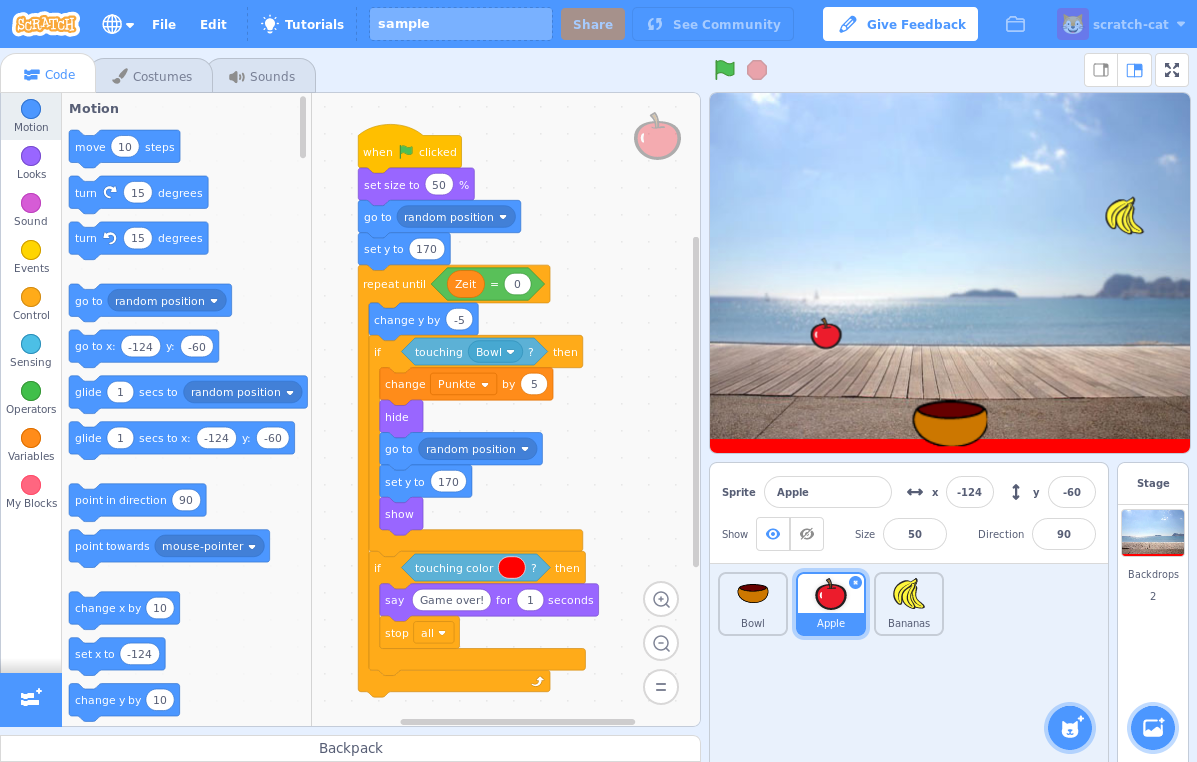
\includegraphics[width=.9\textwidth]{scratch-gui}
        \caption{Scratch's GUI}
    \end{figure}
\end{frame}

\begin{frame}\frametitle{What is Scratch?}
    \begin{itemize}
        \item Block-based programming language
        \item Developed by the MIT media lab
        \item Code is separated into scripts that are triggered by events
    \end{itemize}

    \begin{figure}
        \centering
        \tikzset{>=latex,
                 arrow/.style={-{Latex[length=1.5mm, width=1.5mm]}},
                   box/.style={draw, text width=3.2cm, minimum height=0.7cm, text centered, rounded corners},
                 label/.style={text width=1.9cm}}

        \begin{tikzpicture}[scale=0.8, every node/.style={scale=0.8}]
            \node[box] at (0.0, 1.5) (step)   {Run scripts in parallel until a sprite changes};
            \node[box] at (0.0, 0.0) (render) {Render the stage};

            \node[label] at (-3.5, 1.0) {30 times per second};

            \draw[shorten >= 2pt, arrow, rounded corners]
                   (step)
                -- (render)
                -- ( 0.0, -1.0)
                -- (-2.4, -1.0)
                -- (-2.4,  3.0)
                -- ( 0.0,  3.0)
                -- (step);
        \end{tikzpicture}

        \caption{Scratch step cycle}
    \end{figure}
\end{frame}

\begin{frame}
    \bigcenter{Why Scratch?}
    % Why is Scratch relevant?
    % Scratch is widely popular
    % For one thing, Scratch has a big online community
\end{frame}

\begin{frame}\frametitle{Why Scratch? Scratch's online community}
    % It has an online repository that everyone can upload their own projects to
    \begin{figure}
        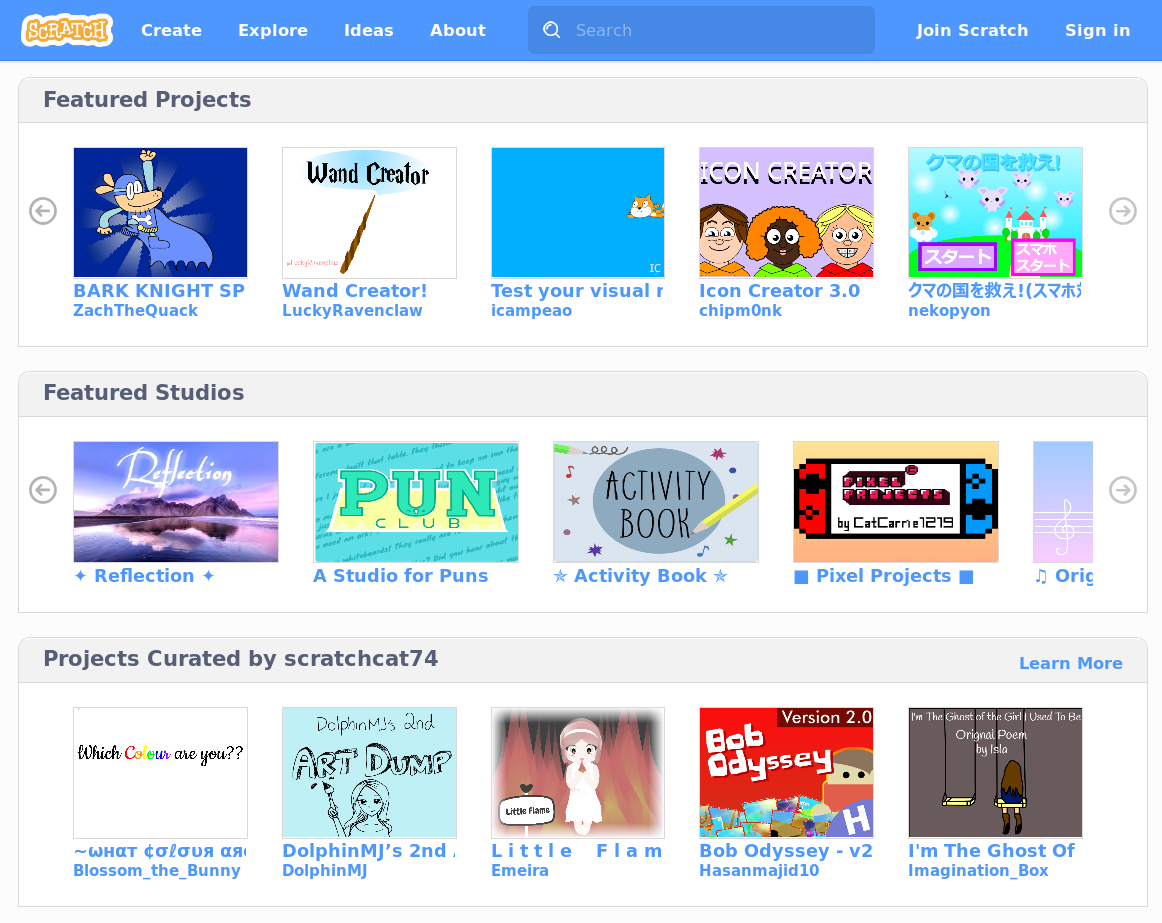
\includegraphics[width=.7\textwidth]{scratch-repository}
        \caption{Scratch's online repository}
    \end{figure}
\end{frame}

\begin{frame}[shrink=0]\frametitle{Why Scratch? Scratch's online community}
    % This repository encompasses over 38 million Scratch projects from over 36 million users at the time of writing
    % With over a million projects uploaded each month
    \begin{figure}
        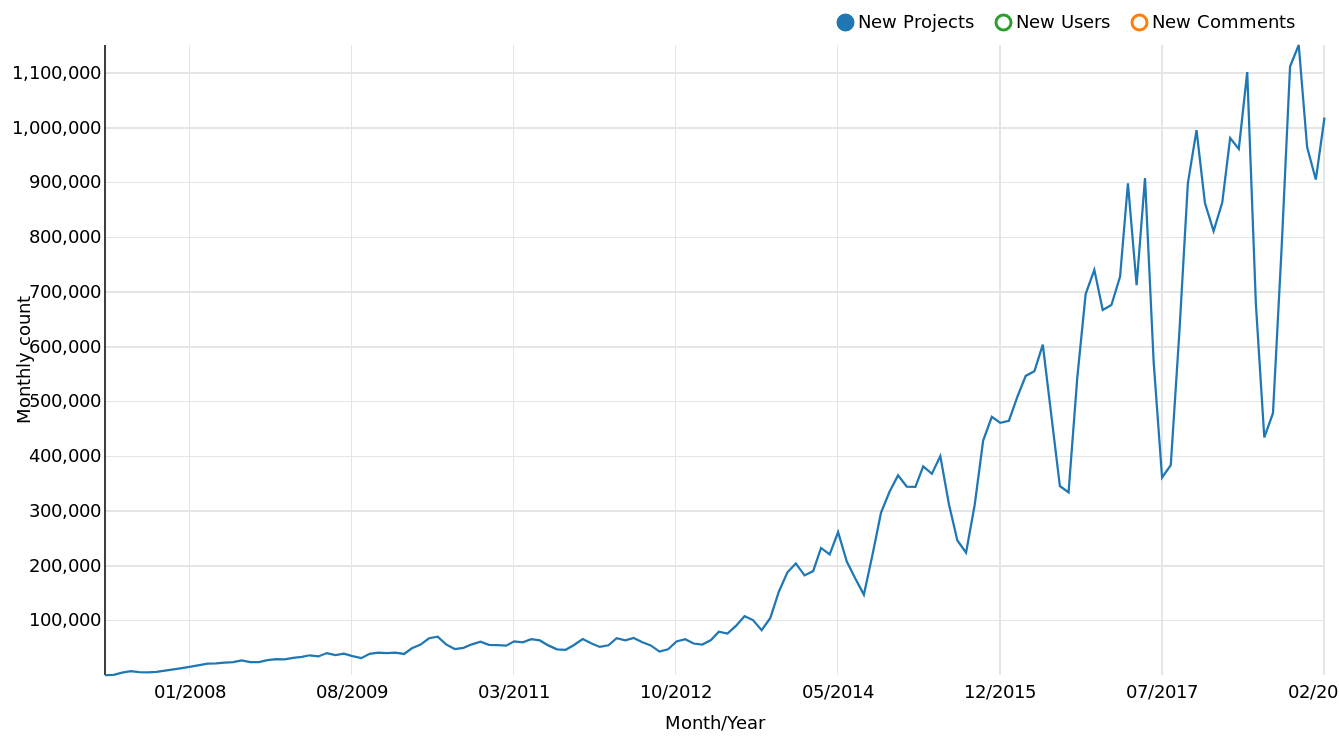
\includegraphics[width=.7\textwidth]{scratch-popularity}
        \caption{Submitted Scratch projects per month}
    \end{figure}
    \centering
    \begin{minipage}{.7\textwidth}
        \begin{itemize}
            \item over 38 million projects shared
            \item over 36 million users
        \end{itemize}
    \end{minipage}
\end{frame}

\begin{frame}\frametitle{Why Scratch? Good introduction to programming}
    % But more importantly Scratch is used by many schools and universities to introduce students to the principles of programming
    % Scratch is very suitable for this task for multiple reasons
    Many schools and universities deploy Scratch as a gentle introduction to programming.
\end{frame}

\begin{frame}\frametitle{Why Scratch? Good introduction to programming}
    % For one thing, Scratch makes it impossible to write invalid code
    % The block-based code system eliminates the possibility of syntax errors
    % Blocks are chosen from a drawer
    % And even variable names can't be misspelled since they are chosen from a list
    % This all helps make Scratch very intuitive to use
    \centering
    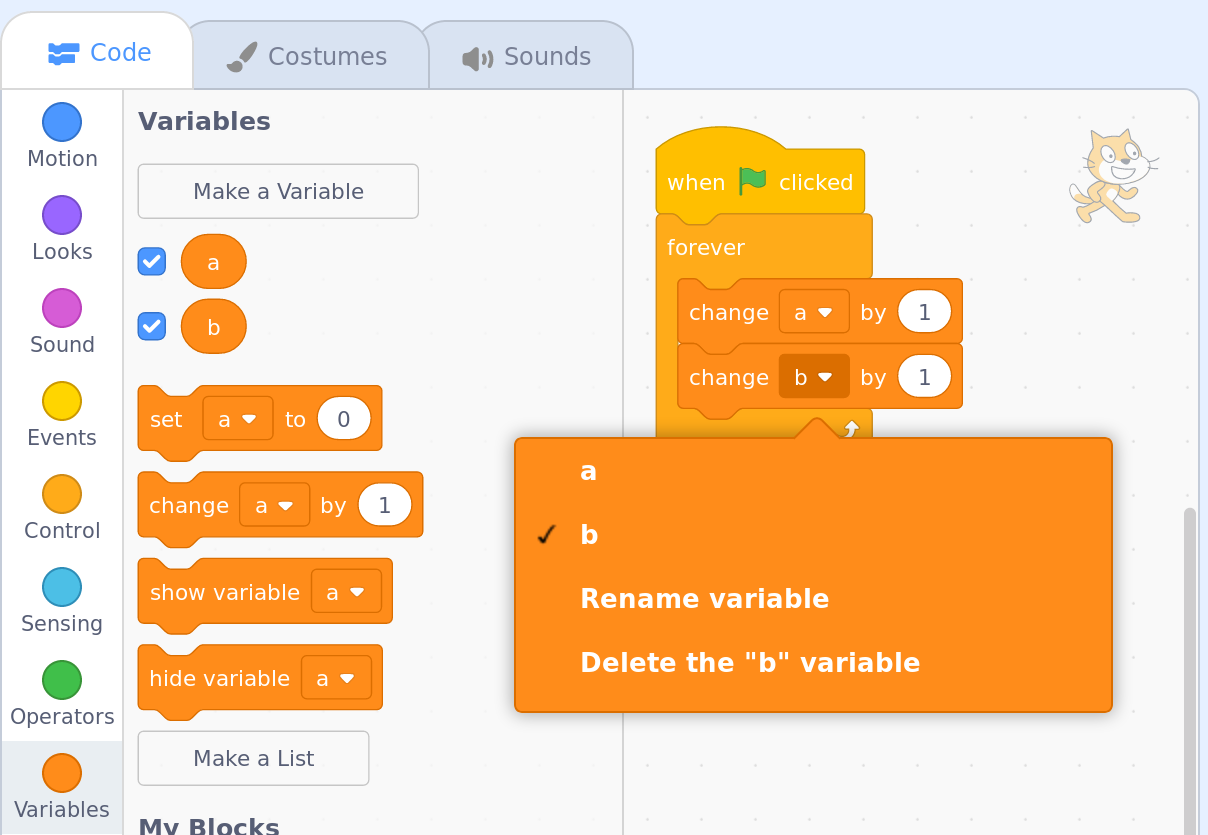
\includegraphics[width=.8\textwidth]{scratch-valid-code}\\[\medskipamount]
    Intuitive: Block based code system only allows valid code
\end{frame}

\begin{frame}\frametitle{Why Scratch? Good introduction to programming}
    % At the same time, Scratch is very engaging
    % User input, graphics and audio are easy to integrate, which often leads to game-like programs
    \centering
    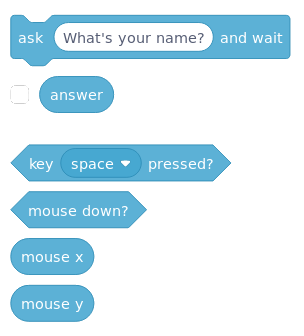
\includegraphics[width=.33\textwidth]{scratch-input-blocks}
    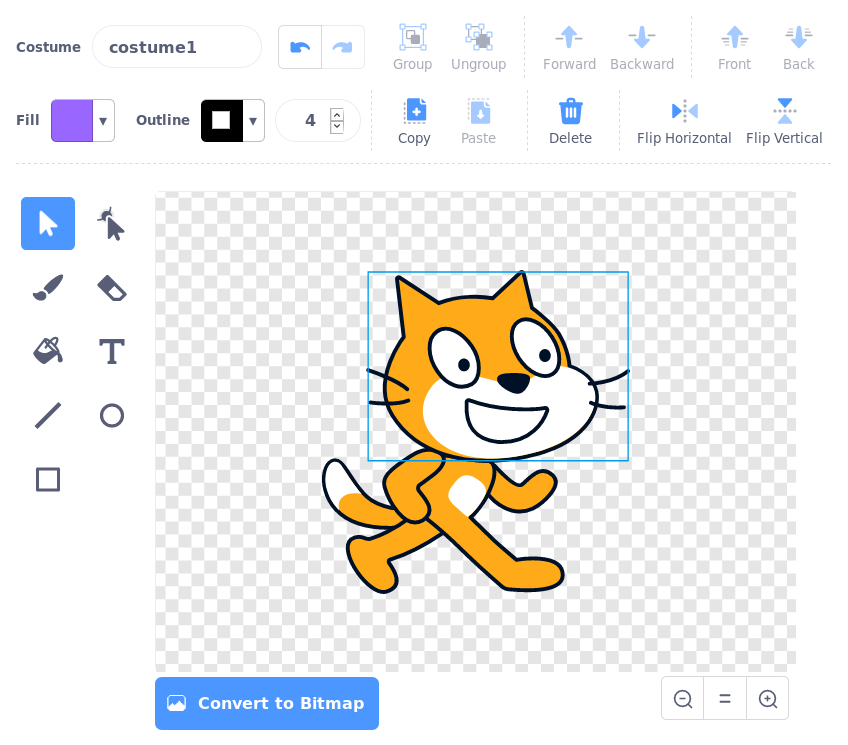
\includegraphics[width=.4\textwidth]{scratch-sprite-editor}
    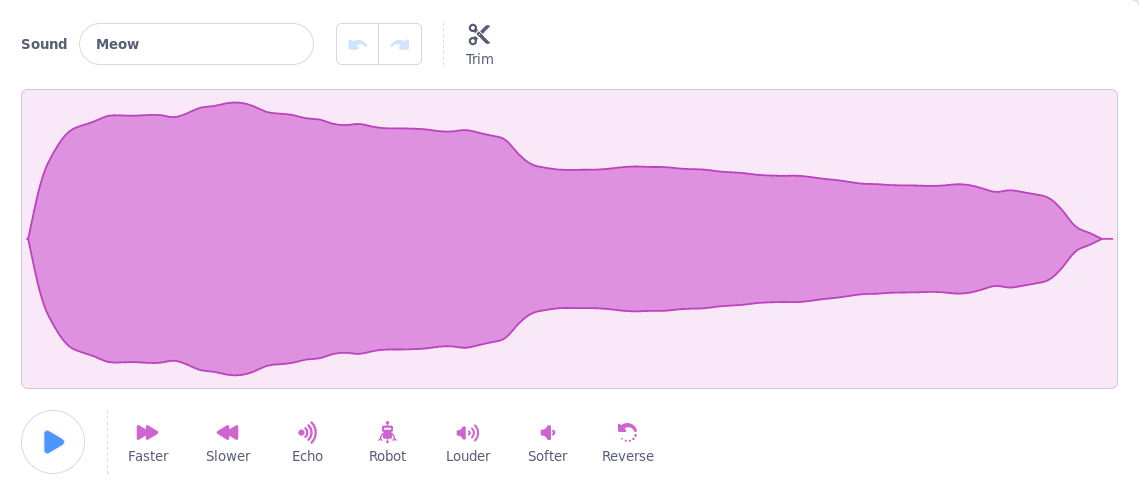
\includegraphics[width=.6\textwidth]{scratch-sound-editor}\\[\medskipamount]
    Engaging: User interaction, easy integration of graphics and sounds
\end{frame}

\begin{frame}
    \bigcenter{Why automated testing for Scratch?}
\end{frame}

\begin{frame}\frametitle{Why automated testing for Scratch?}
    Grading Scratch assignments is very \textcolor{upfim}{time consuming}
    \begin{itemize}
        \item every project has to be opened individually
        \item programs require large amounts of \textcolor{upfim}{user interaction}
    \end{itemize}

    \bigskip

    % TODO citation
    Some courses are attended by a \textcolor{upfim}{large number of students ($> 200$)},
    making manual testing for grading infeasible.

    \bigskip

    Students can also use automated tests to get feedback for their own implementations.
\end{frame}

\begin{frame}
    \bigcenter{Why is automated testing for Scratch difficult?}
\end{frame}

\begin{frame}\frametitle{Why is automated testing for Scratch difficult?}
    Usually functional testing is deployed to automatically assess student solution,
    but this is not straightforward for Scratch
    \begin{itemize}
        \item Scratch is normally only accessible through its GUI
        \item \textcolor{upfim}{no functions} that take parameters and return a value
        \item \textcolor{upfim}{no textual IO}, keyboard and mouse input and graphical output
    \end{itemize}

    \bigskip

    \centering
    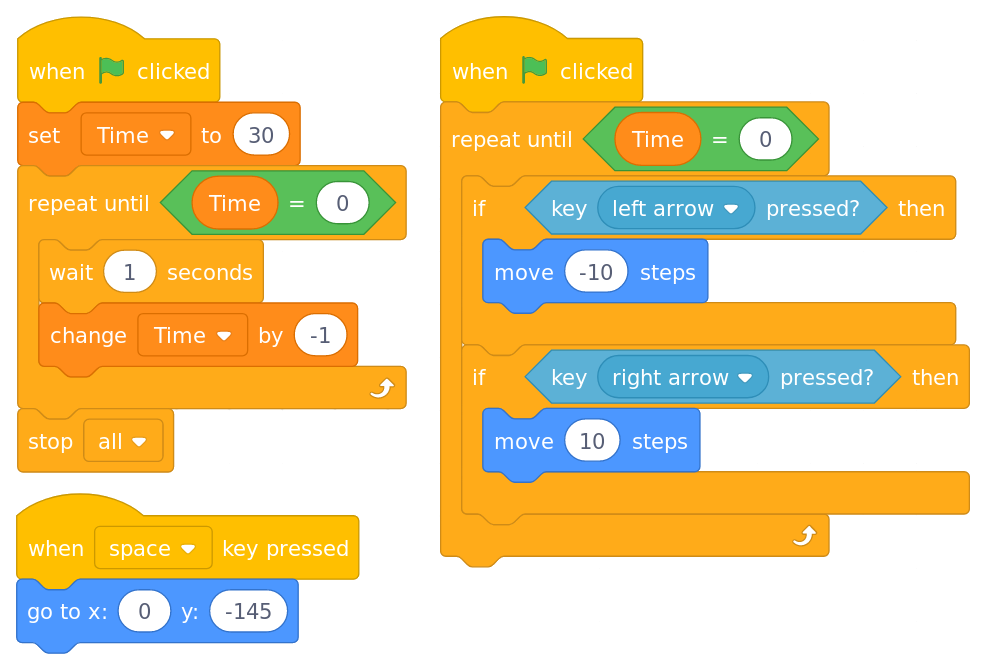
\includegraphics[width=.45\textwidth]{scratch-code}
    \hspace{1em}
    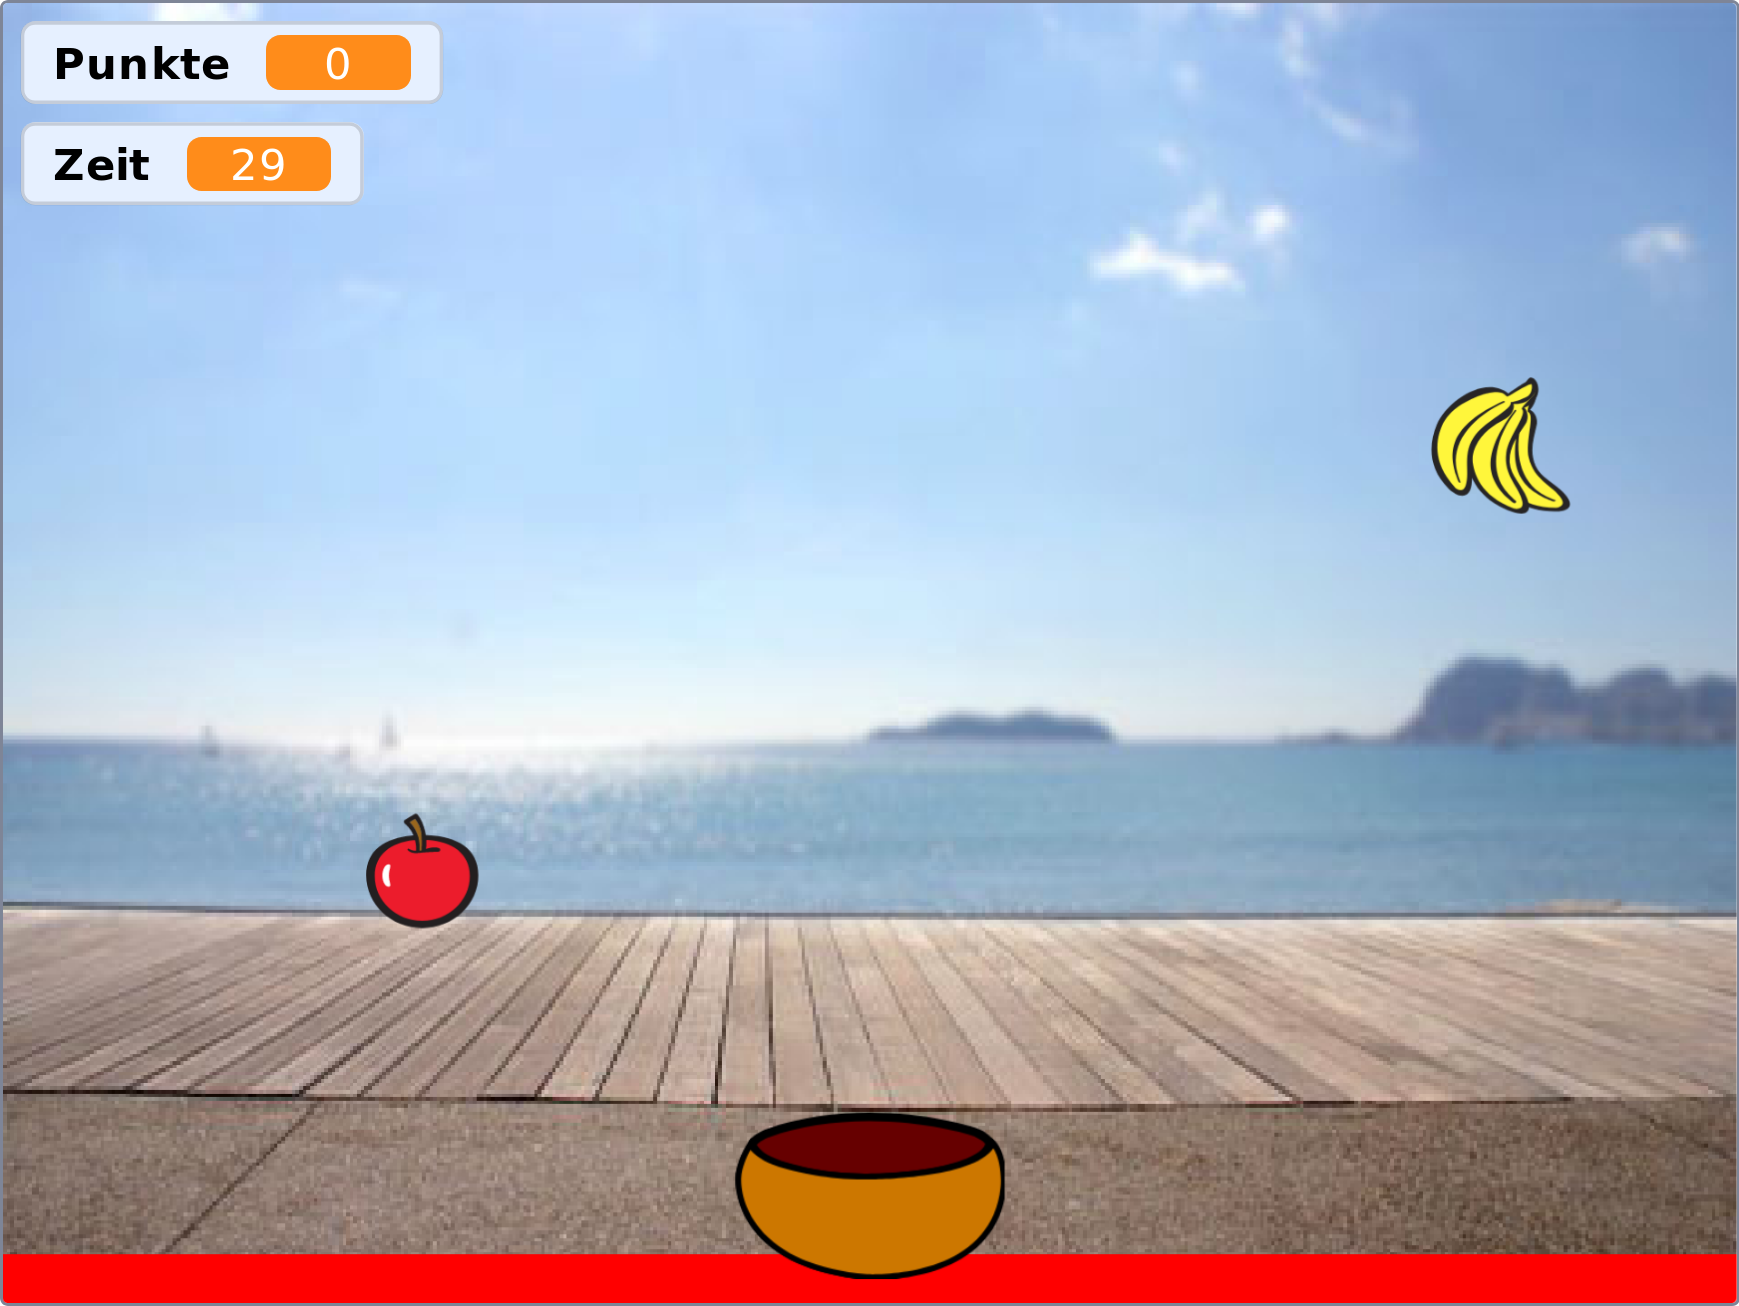
\includegraphics[width=.4\textwidth]{scratch-stage}
\end{frame}

\begin{frame}
    \bigcenter{How to test Scratch programs?}
\end{frame}

\begin{frame}[fragile]\frametitle{How to test Scratch programs? Automating IO}
    Approach: Test on a system level by automating Scratch's IO

    \begin{center}

    \tikzset{>=latex,
           arrow/.style={draw, -{Latex[length=1.5mm, width=1.5mm]}},
             put/.style={draw, minimum height=0.65cm, minimum width=1.75cm, rounded corners, fill=red!20, text width=2.4cm, text centered},
              vm/.style={draw, minimum height=1.75cm, minimum width=3.0cm, rounded corners, fill=white},
             gui/.style={draw, minimum height=2.6cm, minimum width=3.5cm, rounded corners, fill=blue!20},
         whisker/.style={draw, minimum height=2.6cm, minimum width=3.5cm, rounded corners, fill=green!20},
             box/.style={draw,text centered, rounded corners}}

    \hspace{2mm}\begin{tikzpicture}[scale=0.9, every node/.style={scale=0.9}]
        \node[box] at (0.0, 4.0) (input)  {
\includegraphics[height=.25\textheight]{mouse-keyboard}};
        \node[box] at (5.1, 4.0) (output) {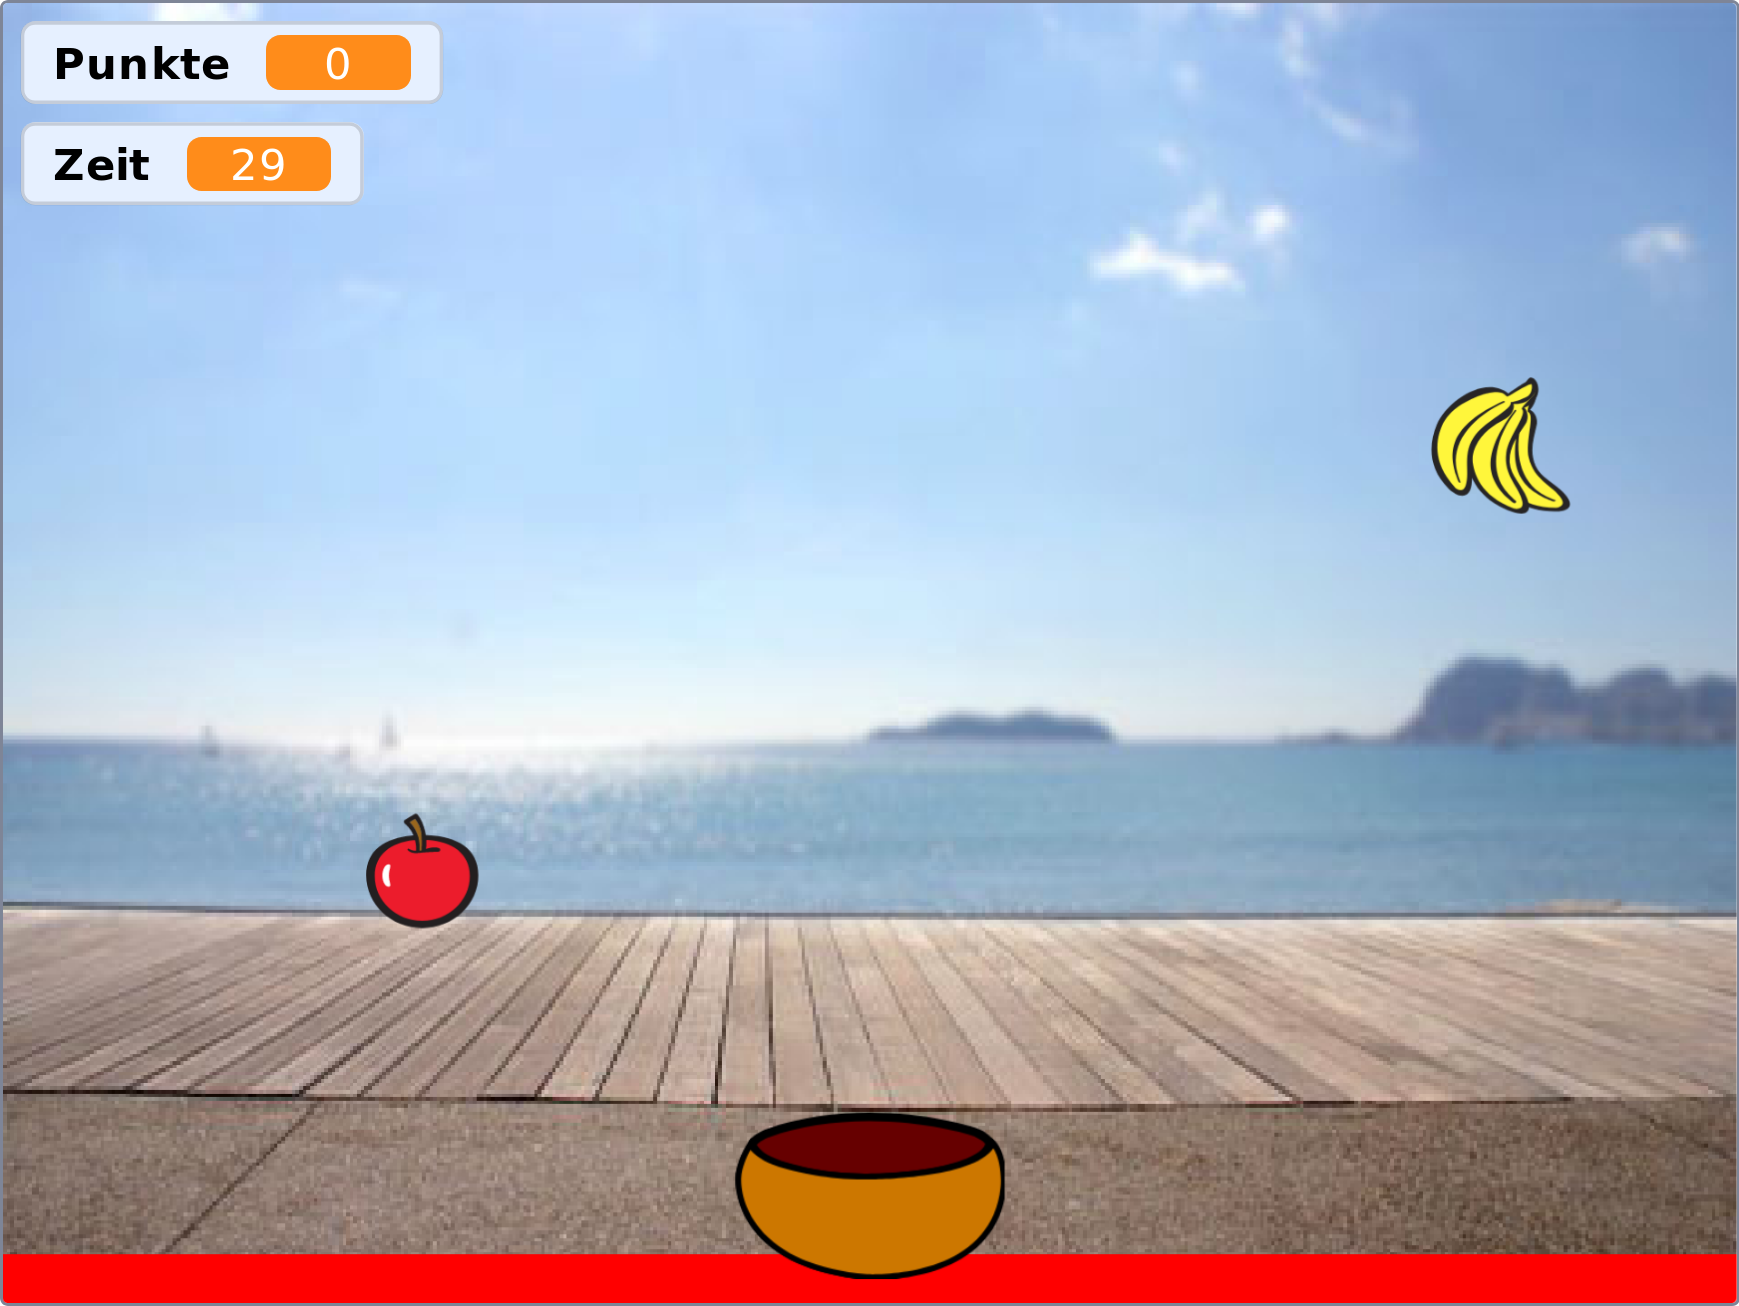
\includegraphics[height=.25\textheight]{scratch-stage}};

        \node[] at (0.0, 5.5) (inputtxt)  {\textbf{Input}};
        \node[] at (5.1, 5.5) (outputtxt) {\textbf{Output}};

        \draw [shorten >= 2pt, shorten <= 2pt, arrow] (input) -- (output);
    \end{tikzpicture}

    \bigskip

    \begin{tikzpicture}[scale=0.9, every node/.style={scale=0.9}]
        \node[box] at (-0.1, 4.0) (input) {
            \begin{minipage}{.28\textwidth}
                \begin{minted}[autogobble, breaklines, fontsize=\scriptsize, frame=none]{javascript}
                    t.inputImmediate({
                        device: 'mouse',
                        isDown: true,
                        x: 50,
                        y: 100
                    });
                \end{minted}
            \end{minipage}
        };

        \node[box] at (5.1, 4.0) (output) {
            \begin{minipage}{.28\textwidth}
                \begin{minted}[autogobble, breaklines, fontsize=\scriptsize, frame=none]{javascript}
                    sprite.x
                    sprite.y
                    sprite.rotation
                    sprite.sayText
                    sprite.costume
                    variable.value
                \end{minted}
            \end{minipage}
        };

        \node[] at (0.0, 5.5) (inputtxt)  {\textbf{Input}};
        \node[] at (5.1, 5.5) (outputtxt) {\textbf{Output}};

        \draw [shorten >= 2pt, shorten <= 2pt, arrow] (input) -- (output);
    \end{tikzpicture}

    \end{center}
\end{frame}

\begin{frame}\frametitle{How to test Scratch programs? Automating IO}
    \begin{figure}
        \centering
        \tikzset{>=latex,
                 arrow/.style={-{Latex[length=1.5mm, width=1.5mm]}},
                 label/.style={draw=none, text width=5.3cm, minimum height=0.5cm, text centered},
                   box/.style={draw,      text width=3.2cm, minimum height=0.7cm, text centered, rounded corners},
                     h/.style={fill=blue!10}}

        \begin{tikzpicture}
            \node[box, h] at ( 0.0, 3.0) (gui)           {Scratch GUI};
            \node[box]    at (-2.0, 1.5) (scratchvm)     {Scratch VM};
            \node[box]    at ( 2.2, 1.5) (scratchrender) {Scratch Renderer};
            \node[box, color=gray]   at (-2.0, 0.0) (program)       {Program};
            \node[box, color=gray]   at ( 2.2, 0.0) (htmlcanvas)    {HTML Canvas};

            \foreach \pp/\pf/\pt in {--/gui/scratchvm,
                                     --/gui/scratchrender,
                                     --/scratchvm/scratchrender,
                                     --/scratchvm/program,
                                     --/scratchrender/htmlcanvas}
            \draw[shorten >= 2pt, arrow] (\pf) \pp (\pt);
        \end{tikzpicture}

        \caption{General architecture of Scratch}
    \end{figure}
\end{frame}

\begin{frame}\frametitle{How to test Scratch programs? Automating IO}
    \begin{figure}[htpb]
        \centering
        \tikzset{>=latex,
                 arrow/.style={-{Latex[length=1.5mm, width=1.5mm]}},
                 label/.style={draw=none, text width=5.3cm, minimum height=0.5cm, text centered},
                   box/.style={draw,      text width=3.2cm, minimum height=0.7cm, text centered, rounded corners},
                     h/.style={fill=blue!10}}

        \begin{tikzpicture}
            \node[box]    at ( 0.00,  1.5) (testcode)      {Test Code};
            \node[box, h] at ( 0.00,  0.0) (whisker)       {Whisker};
            \node[box]    at (-2.00, -1.5) (scratchvm)     {Scratch VM};
            \node[box]    at ( 2.20, -1.5) (scratchrender) {Scratch Renderer};
            \node[box, color=gray]   at (-2.0, -3.0) (program)       {Program};
            \node[box, color=gray]   at ( 2.2, -3.0) (htmlcanvas)    {HTML Canvas};

            \foreach \pp/\pf/\pt in {--/testcode/whisker,
                                     --/whisker/scratchvm,
                                     --/whisker/scratchrender,
                                     --/scratchvm/scratchrender,
                                     --/scratchvm/program,
                                     --/scratchrender/htmlcanvas}
            \draw[shorten >= 2pt, arrow] (\pf) \pp (\pt);
        \end{tikzpicture}

        \caption{General architecture of Whisker}
    \end{figure}
\end{frame}

\begin{frame}[fragile]\frametitle{How to test Scratch programs? Automating IO}
    \tikzset{>=latex,
           arrow/.style={draw, -{Latex[length=1.5mm, width=1.5mm]}},
             put/.style={draw, minimum height=0.65cm, minimum width=1.75cm, rounded corners, fill=red!20, text width=2.4cm, text centered},
              vm/.style={draw, minimum height=1.75cm, minimum width=3.0cm, rounded corners, fill=white},
             gui/.style={draw, minimum height=2.6cm, minimum width=3.5cm, rounded corners, fill=blue!20},
         whisker/.style={draw, minimum height=2.6cm, minimum width=3.5cm, rounded corners, fill=green!20},
             box/.style={draw,text centered, rounded corners}}

    \hspace{2mm}\begin{tikzpicture}[scale=0.9, every node/.style={scale=0.9}]
        \node[box] at (0.0, 4.0) (input)  {
\includegraphics[height=.25\textheight]{mouse-keyboard}};
        \node[box] at (8.1, 4.0) (output) {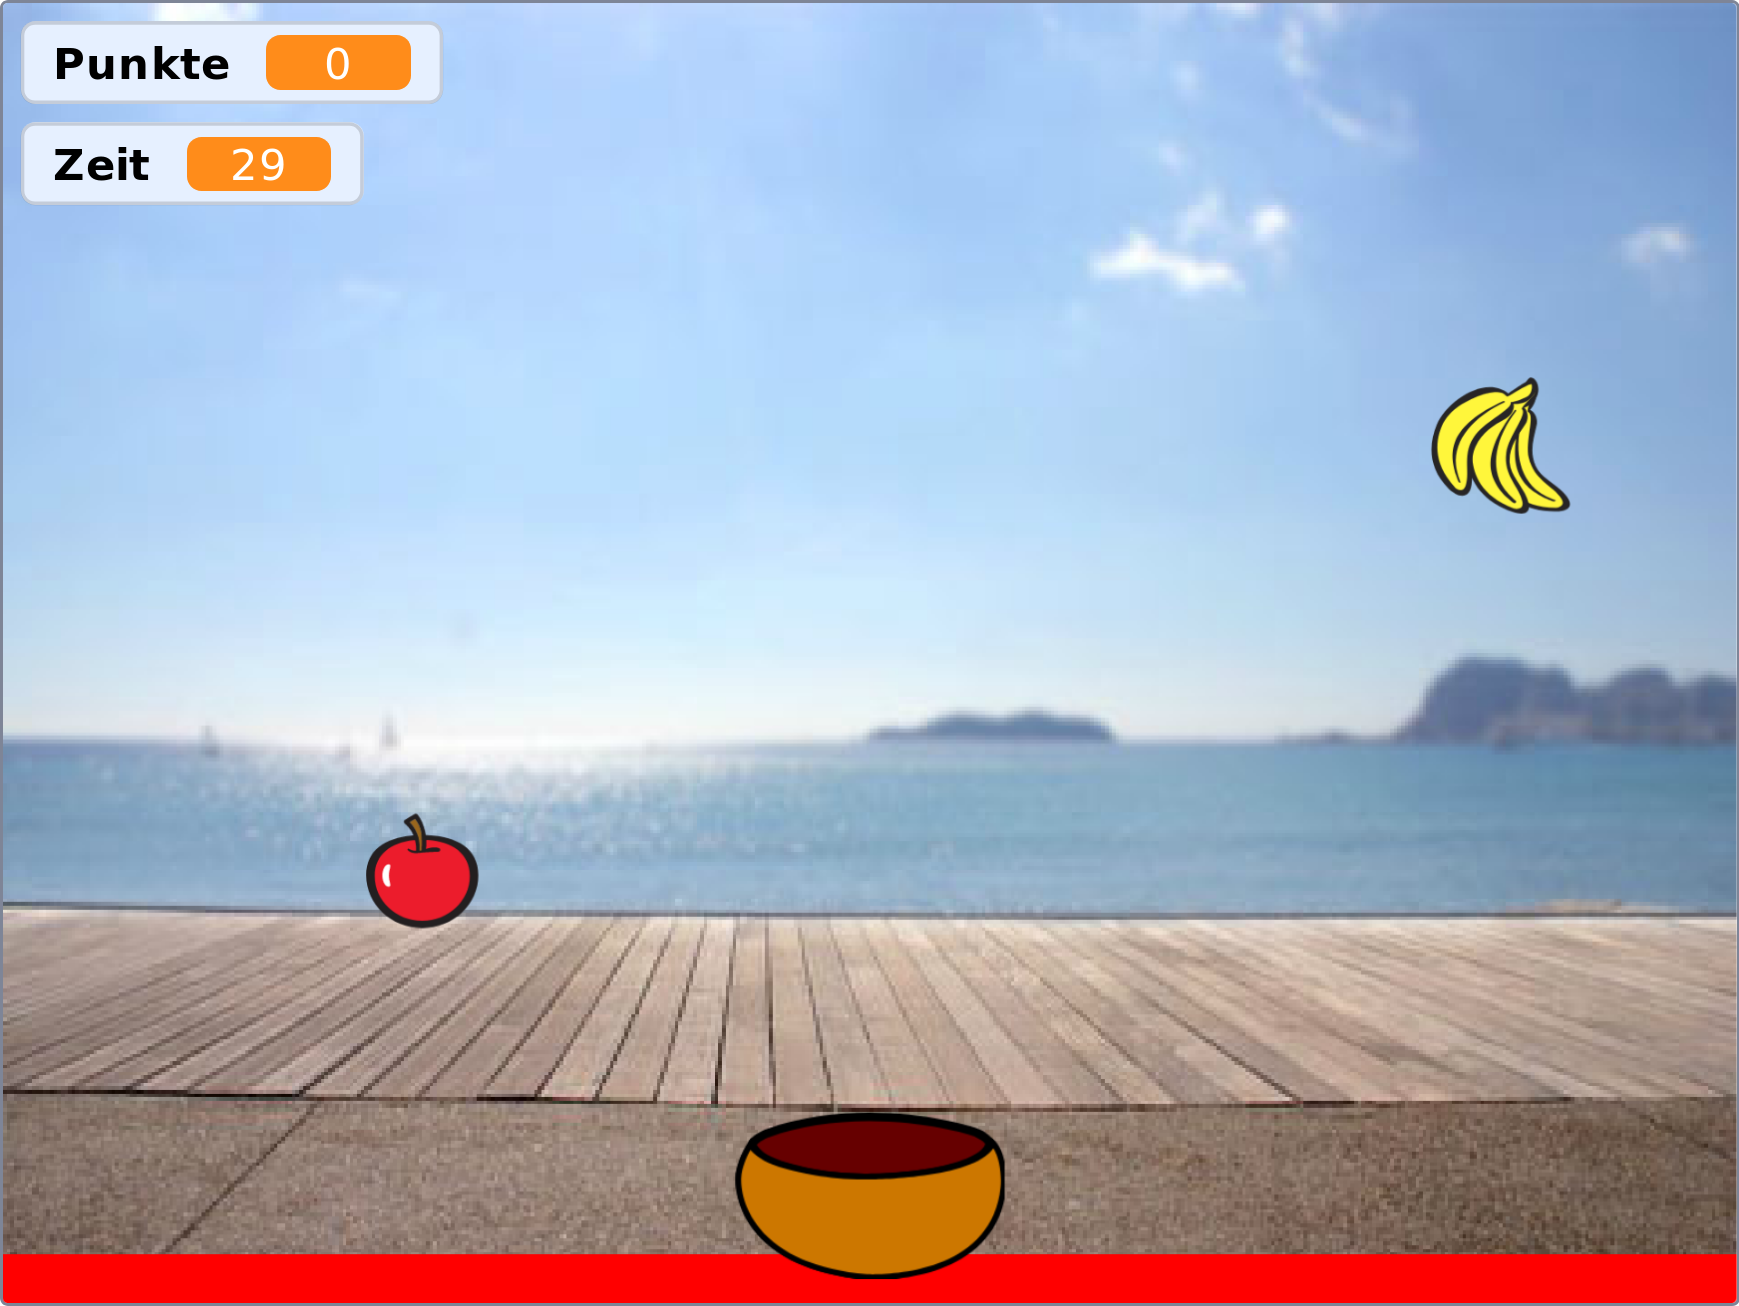
\includegraphics[height=.25\textheight]{scratch-stage}};

        \node[] at (0.0, 5.5) (inputtxt)  {\textbf{Input}};
        \node[] at (8.1, 5.5) (outputtxt) {\textbf{Output}};

        \begin{scope}[on background layer]
            \node[gui] at (4.0,  4.0)  (gui) {};
            \node[vm]  at (4.0,  3.75) (vm)  {};
        \end{scope}

        \node[put] at (4.0,  3.5) (put)     {\small Program under test};
        \node[]    at (4.0,  4.3) (vmtxt)   {\small Scratch VM};
        \node[]    at (4.0,  4.95) (guitxt) {\textbf{Scratch GUI}};

        \draw [shorten >= 2pt, shorten <= 2pt, arrow] (input) -- (gui);
        \draw [shorten >= 2pt, shorten <= 2pt, arrow] (gui)   -- (output);
    \end{tikzpicture}

    \bigskip

    \begin{tikzpicture}[scale=0.9, every node/.style={scale=0.9}]
        \node[box] at (-0.1, 4.0) (input) {
            \begin{minipage}{.28\textwidth}
                \begin{minted}[autogobble, breaklines, fontsize=\scriptsize, frame=none]{javascript}
                    t.inputImmediate({
                        device: 'mouse',
                        isDown: true,
                        x: 50,
                        y: 100
                    });
                \end{minted}
            \end{minipage}
        };

        \node[box] at (8.1, 4.0) (output) {
            \begin{minipage}{.28\textwidth}
                \begin{minted}[autogobble, breaklines, fontsize=\scriptsize, frame=none]{javascript}
                    sprite.x
                    sprite.y
                    sprite.rotation
                    sprite.sayText
                    sprite.costume
                    variable.value
                \end{minted}
            \end{minipage}
        };

        \node[] at (0.0, 5.4) (inputtxt)  {\textbf{Input}};
        \node[] at (8.1, 5.4) (outputtxt) {\textbf{Output}};

        \begin{scope}[on background layer]
            \node[whisker] at (4.0,  4.0)  (whisker) {};
            \node[vm]      at (4.0,  3.75) (vm)      {};
        \end{scope}

        \node[put] at (4.0,  3.5)  (put)        {\small Program under test};
        \node[]    at (4.0,  4.3)  (vmtxt)      {\small Scratch VM};
        \node[]    at (4.0,  4.95) (whiskertxt) {\textbf{Whisker}};

        \draw [shorten >= 2pt, shorten <= 2pt, arrow] (input)   -- (whisker);
        \draw [shorten >= 2pt, shorten <= 2pt, arrow] (whisker) -- (output);
    \end{tikzpicture}
\end{frame}

\begin{frame}
    \bigcenter{Whisker}
\end{frame}

\begin{frame}\frametitle{Whisker, Whisker's GUI}
    \begin{figure}
        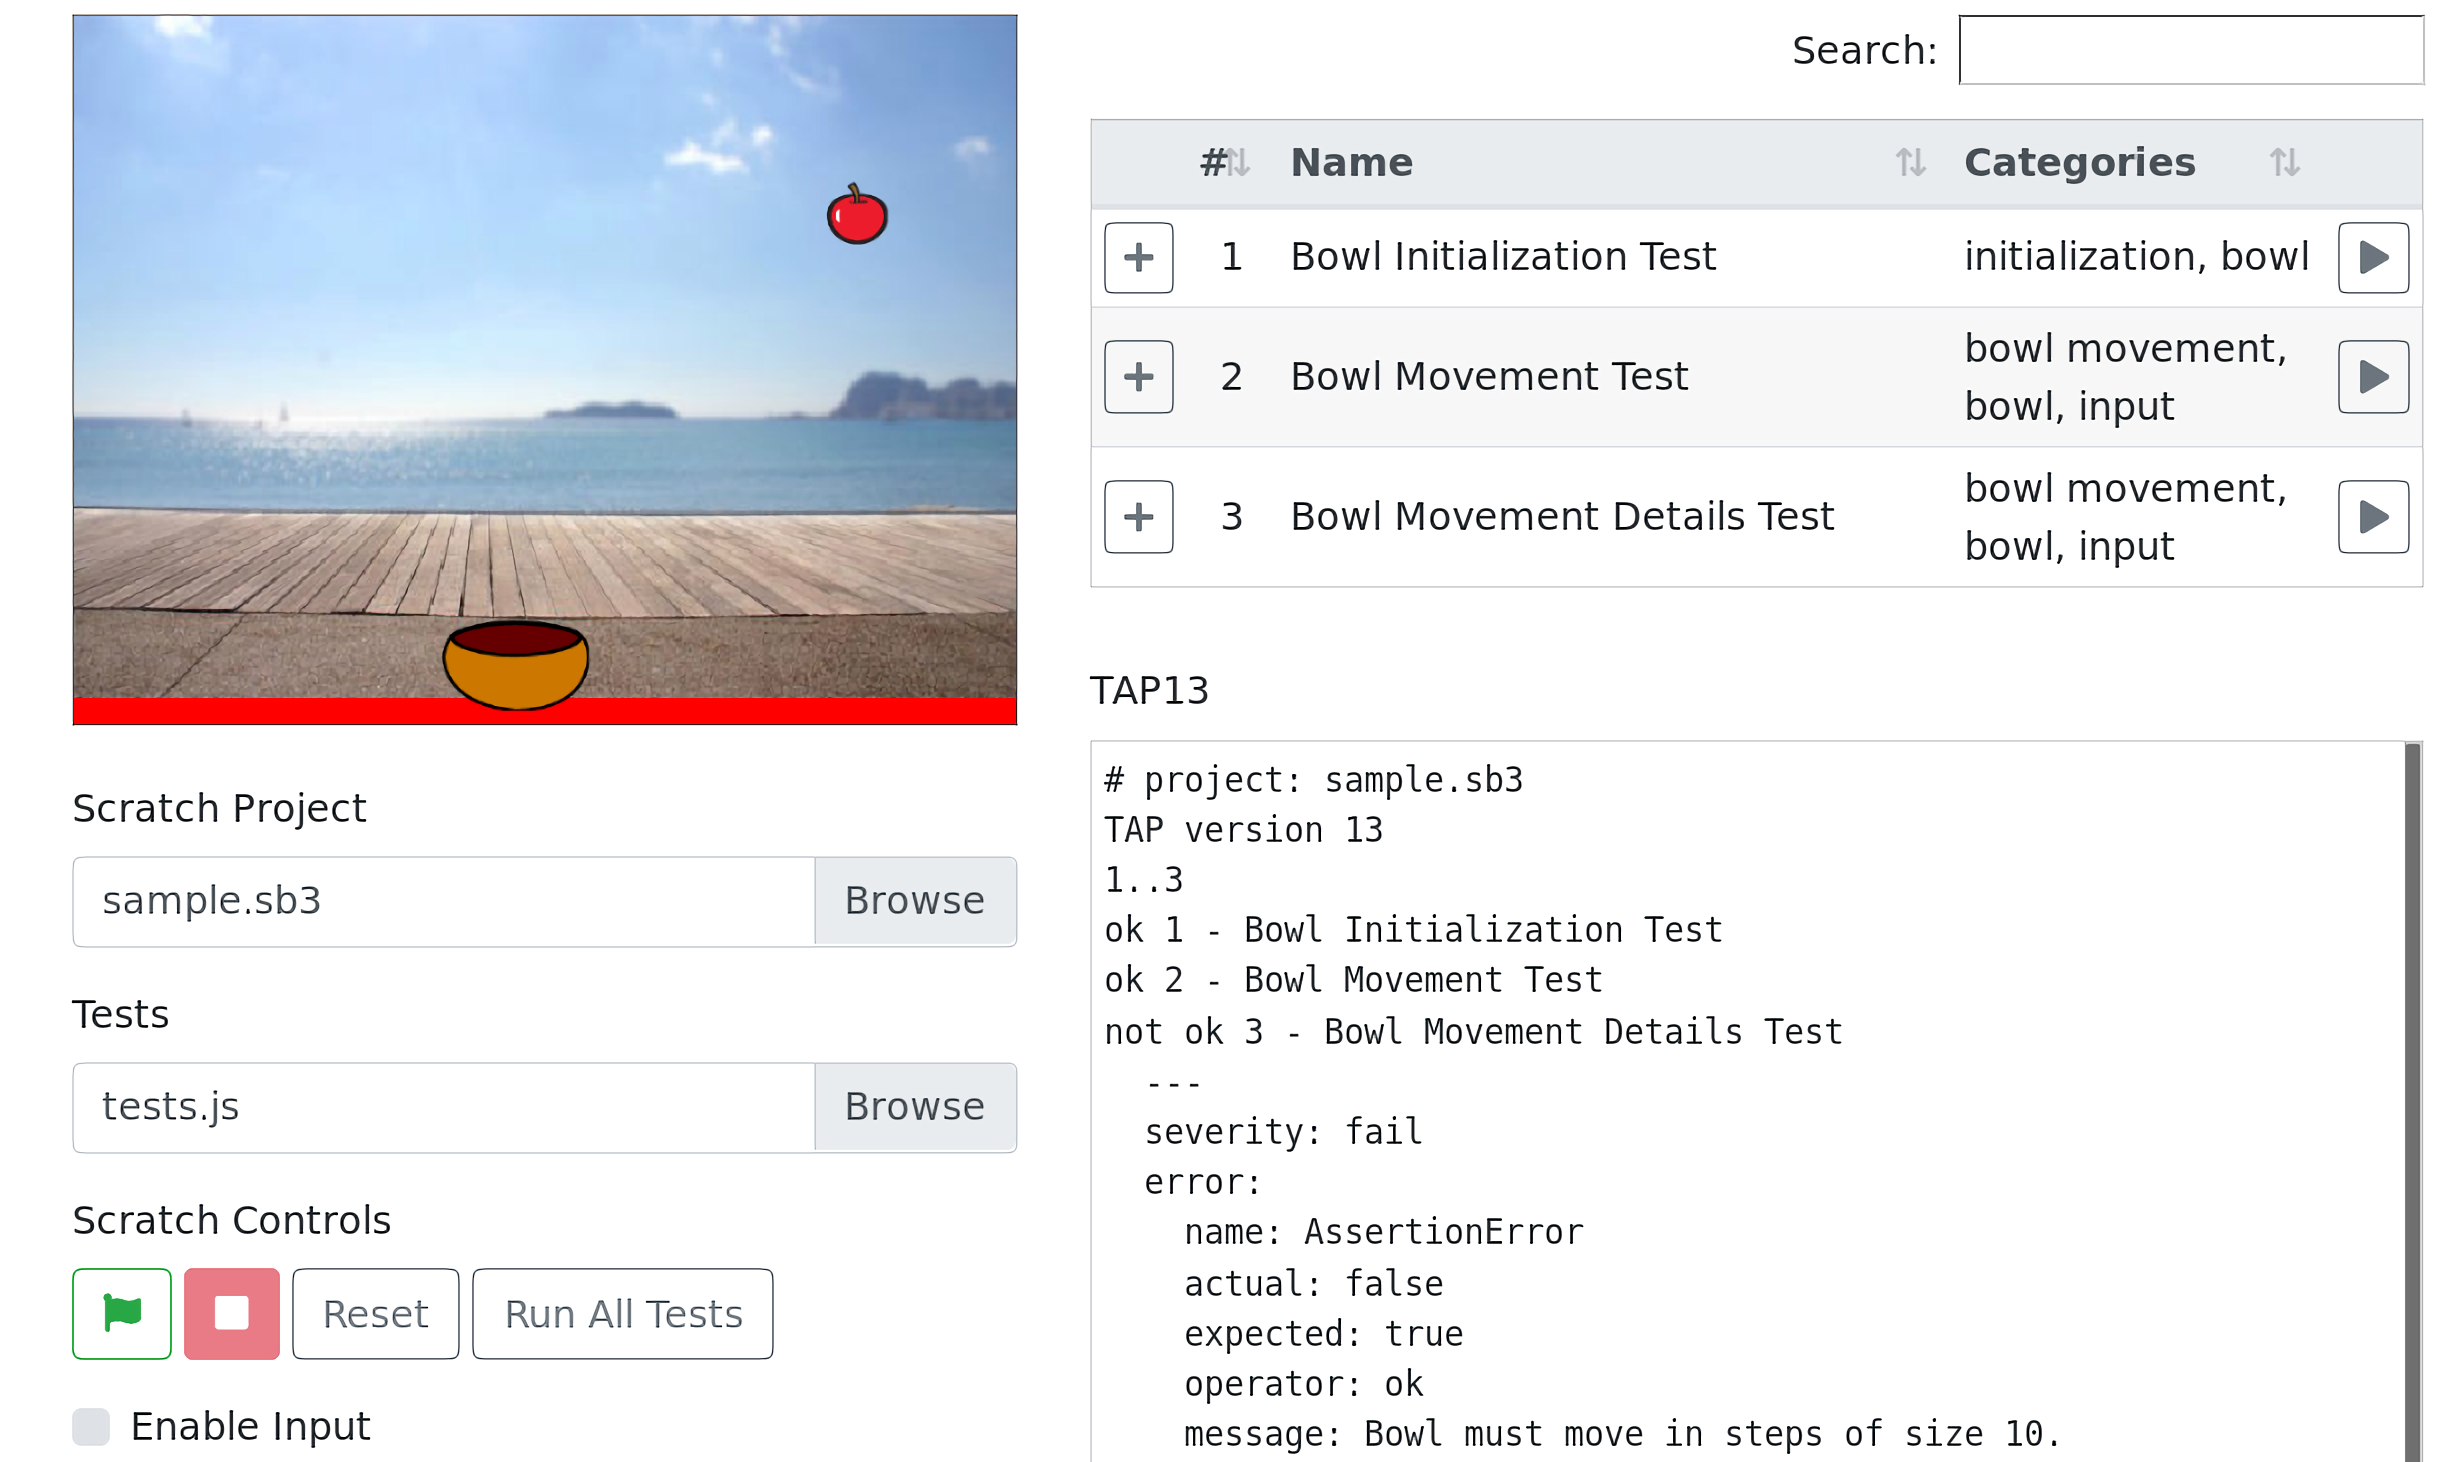
\includegraphics[width=\textwidth]{whisker-gui-big-upscaled}
        \caption{Whisker's GUI}
    \end{figure}
    % Whisker allows us to interact with the Scratch VM through a JavaScript API
\end{frame}

\begin{frame}[fragile]\frametitle{Whisker, Example Test}
    \vspace{-\bigskipamount}
    \begin{minipage}{.7\textwidth}\begin{tikzpicture}
        \node[opacity=1.0] (0,0) {
            \begin{minipage}{\textwidth}
                \begin{javascriptcode}
                    const test = async function (t) {
                        const sprite = t.getSprite('Sprite1');

                        await t.runForTime(100);
                        let oldX = sprite.x;

                        await t.runForTime(1000);

                        t.assert.ok(oldX === sprite.x);

                        t.inputImmediate({
                            device: 'keyboard',
                            key: 'right arrow',
                            isDown: true
                        });

                        await t.runForTime(1000);

                        t.assert.ok(oldX < sprite.x);
                    }
                \end{javascriptcode}
            \end{minipage}
        };
    \end{tikzpicture}\end{minipage}
\end{frame}

\begin{frame}[fragile]\frametitle{Whisker, Accessing Sprites and Variables}
    \vspace{-\bigskipamount}
    \begin{minipage}{.7\textwidth}\begin{tikzpicture}
        \node[opacity=0.35] (0,0) {
            \begin{minipage}{\textwidth}
                \begin{javascriptcode}
                    const test = async function (t) {
                        const sprite = t.getSprite('Sprite1');

                        await t.runForTime(100);
                        let oldX = sprite.x;

                        await t.runForTime(1000);

                        t.assert.ok(oldX === sprite.x);

                        t.inputImmediate({
                            device: 'keyboard',
                            key: 'right arrow',
                            isDown: true
                        });

                        await t.runForTime(1000);

                        t.assert.ok(oldX < sprite.x);
                    }
                \end{javascriptcode}
            \end{minipage}
        };
    \end{tikzpicture}\end{minipage}%
    \hspace{-.4\textwidth}%
    \begin{minipage}{.6\textwidth}
        \begin{javascriptcode}
            t.getSprite('Sprite1');
            t.getSprites(sprite => sprite.x > 100);
            t.getStage();

            sprite.getClones();
            sprite.getVariable('my variable');

            sprite.x;
            sprite.rotation;
            variable.value;

            sprite.old.x;
            sprite.old.rotation;
            variable.old.value;

            sprite.isTouchingEdge();
        \end{javascriptcode}
    \end{minipage}
\end{frame}

\begin{frame}[fragile]\frametitle{Whisker, Example Test}
    \vspace{-\bigskipamount}
    \begin{minipage}{.7\textwidth}\begin{tikzpicture}
        \node[opacity=1.0] (0,0) {
            \begin{minipage}{\textwidth}
                \begin{javascriptcode}
                    const test = async function (t) {
                        const sprite = t.getSprite('Sprite1');

                        await t.runForTime(100);
                        let oldX = sprite.x;

                        await t.runForTime(1000);

                        t.assert.ok(oldX === sprite.x);

                        t.inputImmediate({
                            device: 'keyboard',
                            key: 'right arrow',
                            isDown: true
                        });

                        await t.runForTime(1000);

                        t.assert.ok(oldX < sprite.x);
                    }
                \end{javascriptcode}
            \end{minipage}
        };
    \end{tikzpicture}\end{minipage}
\end{frame}

\begin{frame}[fragile]\frametitle{Whisker, Running the Program}
    \vspace{-\bigskipamount}
    \begin{minipage}{.7\textwidth}\begin{tikzpicture}
        \node[opacity=0.35] (0,0) {
            \begin{minipage}{\textwidth}
                \begin{javascriptcode}
                    const test = async function (t) {
                        const sprite = t.getSprite('Sprite1');

                        await t.runForTime(100);
                        let oldX = sprite.x;

                        await t.runForTime(1000);

                        t.assert.ok(oldX === sprite.x);

                        t.inputImmediate({
                            device: 'keyboard',
                            key: 'right arrow',
                            isDown: true
                        });

                        await t.runForTime(1000);

                        t.assert.ok(oldX < sprite.x);
                    }
                \end{javascriptcode}
            \end{minipage}
        };
    \end{tikzpicture}\end{minipage}%
    \hspace{-.4\textwidth}%
    \begin{minipage}{.6\textwidth}
        \begin{javascriptcode}
            await t.runForTime(1000);
            await t.runUntil(() => a > b, 1000);

            t.getRunTimeElapsed();
            t.getTotalTimeElapsed();

            t.greenFlag();
        \end{javascriptcode}
    \end{minipage}
\end{frame}

\begin{frame}[fragile]\frametitle{Whisker, Example Test}
    \vspace{-\bigskipamount}
    \begin{minipage}{.7\textwidth}\begin{tikzpicture}
        \node[opacity=1.0] (0,0) {
            \begin{minipage}{\textwidth}
                \begin{javascriptcode}
                    const test = async function (t) {
                        const sprite = t.getSprite('Sprite1');

                        await t.runForTime(100);
                        let oldX = sprite.x;

                        await t.runForTime(1000);

                        t.assert.ok(oldX === sprite.x);

                        t.inputImmediate({
                            device: 'keyboard',
                            key: 'right arrow',
                            isDown: true
                        });

                        await t.runForTime(1000);

                        t.assert.ok(oldX < sprite.x);
                    }
                \end{javascriptcode}
            \end{minipage}
        };
    \end{tikzpicture}\end{minipage}
\end{frame}

\begin{frame}[fragile]\frametitle{Whisker, Simulating Inputs}
    \vspace{-\bigskipamount}
    \begin{minipage}{.7\textwidth}\begin{tikzpicture}
        \node[opacity=0.35] (0,0) {
            \begin{minipage}{\textwidth}
                \begin{javascriptcode}
                    const test = async function (t) {
                        const sprite = t.getSprite('Sprite1');

                        await t.runForTime(100);
                        let oldX = sprite.x;

                        await t.runForTime(1000);

                        t.assert.ok(oldX === sprite.x);

                        t.inputImmediate({
                            device: 'keyboard',
                            key: 'right arrow',
                            isDown: true
                        });

                        await t.runForTime(1000);

                        t.assert.ok(oldX < sprite.x);
                    }
                \end{javascriptcode}
            \end{minipage}
        };
    \end{tikzpicture}\end{minipage}%
    \hspace{-.4\textwidth}%
    \begin{minipage}{.6\textwidth}
        \begin{javascriptcode}
            t.inputImmediate({
                device: 'keyboard',
                key: 'right arrow',
                isDown: true,
                duration: 100
            });
            t.addInput(1000, {
                device: 'mouse',
                x: 100, y: 200,
                isDown: true
            });
            t.addInput(2000, {
                device: 'text',
                text: 'some answer'
            });

            t.getMousePos();
            t.isKeyDown('space');
        \end{javascriptcode}
    \end{minipage}
\end{frame}

\begin{frame}[fragile]\frametitle{Whisker, Example Test}
    \vspace{-\bigskipamount}
    \begin{minipage}{.7\textwidth}\begin{tikzpicture}
        \node[opacity=1.0] (0,0) {
            \begin{minipage}{\textwidth}
                \begin{javascriptcode}
                    const test = async function (t) {
                        const sprite = t.getSprite('Sprite1');

                        await t.runForTime(100);
                        let oldX = sprite.x;

                        await t.runForTime(1000);

                        t.assert.ok(oldX === sprite.x);

                        t.inputImmediate({
                            device: 'keyboard',
                            key: 'right arrow',
                            isDown: true
                        });

                        await t.runForTime(1000);

                        t.assert.ok(oldX < sprite.x);
                    }
                \end{javascriptcode}
            \end{minipage}
        };
    \end{tikzpicture}\end{minipage}
\end{frame}

\begin{frame}[fragile]\frametitle{Whisker, Callbacks}
    \begin{itemize}
        \item Callbacks get executed every time a frame is rendered
        \item Make it possible to \textcolor{upfim}{track} and \textcolor{upfim}{react} to what the user sees
    \end{itemize}

    \begin{javascriptcode}
        t.addCallback(() => someList.push(sprite.x));

        const callback = t.addCallback(() => {
            if (sprite.visible) {
                t.inputImmediate({ device: 'mouse', isDown: true });
            } else {
                t.inputImmediate({ device: 'mouse', isDown: false });
            }
        });

        callback.disable();
        callback.enable();
        callback.isActive();
    \end{javascriptcode}
    % TODO: remove disable / enable / isActive
\end{frame}

\begin{frame}[fragile]\frametitle{Whisker, Constraints}
    \begin{itemize}
        \item Constraints \textcolor{upfim}{define conditions} that must hold for the program
        \item Like callbacks, constraints are checked (executed) every time a frame is rendered
    \end{itemize}

    \begin{javascriptcode}
        t.onConstraintFailure('fail');
        t.onConstraintFailure('nothing');

        const constraint = t.addConstraint(() => {
            t.assert.ok(sprite.visible === true,
                        'Sprite must always be visible.');
        });

        constraint.disable();
        constraint.enable();
        constraint.isActive();
    \end{javascriptcode}
    % TODO: remove disable / enable / isActive
\end{frame}

\begin{frame}[fragile]\frametitle{Whisker, Automated Input Generation}
    \begin{itemize}
        \item At a constant frequency, performs a random input from a pool
        \item Whisker can detect what inputs the program can react to
    \end{itemize}

    \begin{javascriptcode}
        t.setRandomInputInterval(150);

        t.registerRandomInputs([
          { device: 'keyboard', key: 'left arrow', duration: [50, 100] },
          { device: 'keyboard', key: 'right arrow', duration: [50, 100] },
          { device: 'mouse', x: [-100, 100], y: [-100, 100], weight: 0.5 }
        ]);

        t.detectRandomInputs({ duration: [50, 100] });
    \end{javascriptcode}
\end{frame}

\newcommand{\tablebox}[1]{
    \begin{tikzpicture}
         \node[draw, text width=7.5cm, minimum height=0.6cm, rounded corners] {\footnotesize #1};
    \end{tikzpicture}
}

\begin{frame}\frametitle{Whisker, Detecting Inputs}
    \scalebox{0.75}{
        \begin{tabular}{m{5.25cm}m{9.0cm}}
            \large Scratch Block(s) & \large Resulting Input(s) \\
            \vspace{3.5mm}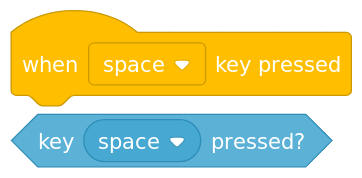
\includegraphics[scale=1.5]{scratch-input-blocks-1}\vspace{2mm} & \tablebox{(1) Press the respective keyboard key}                \\
            \vspace{3.5mm}
\includegraphics[scale=1.5]{scratch-input-blocks-4}\vspace{2mm} & \tablebox{(1) Move the cursor near / onto the respective sprite \\
                                                                                                      (2) Move the cursor to a random position}             \\
            \vspace{3.5mm}
\includegraphics[scale=1.5]{scratch-input-blocks-7}\vspace{2mm} & \tablebox{(1) Answer with a randomly generated string}          \\
            \vspace{3.5mm}
\includegraphics[scale=1.5]{scratch-input-blocks-8}\vspace{2mm} & \tablebox{(1) Answer with the compared string constant}         \\
            \huge ...                                                                     & \huge ...                                                       \\
        \end{tabular}
    }
\end{frame}

\begin{frame}
    \bigcenter{Property-based Testing with Whisker}
\end{frame}

\begin{frame}[fragile]\frametitle{Property-based Testing with QuickCheck}
    Example: QuickCheck

    \medskip

    \begin{itemize}
        \item Define properties
        \item Feed program with (random) input
        \item Check if the program complies to the defined properties
    \end{itemize}

    \pause
    \medskip

    \begin{figure}
        \begin{minted}[autogobble, breaklines, fontsize=\scriptsize, frame=single]{haskell}
            prop_RevApp xs ys =
                reverse (xs++ys) == reverse xs++reverse ys
        \end{minted}

        \begin{minted}[autogobble, breaklines, fontsize=\scriptsize, frame=single]{bash}
            Main> quickCheck prop_RevApp
            OK: passed 100 tests.
        \end{minted}

        \begin{minted}[autogobble, breaklines, fontsize=\scriptsize, frame=single]{bash}
            Main> quickCheck prop_RevApp
            Falsifiable, after 1 tests:
            [2]
            [-2,1]
        \end{minted}

        \caption{QuickCheck Usage Example (from~\cite{quickcheck})}
    \end{figure}
\end{frame}

\begin{frame}\frametitle{Property-based Testing with Whisker}
    Property-based testing can be performed on Scratch programs:
    \begin{itemize}
        \item \textcolor{upfim}{Callbacks:} Observe the program's output
        \item \textcolor{upfim}{Constraints}: Define properties, checked in the background
        \item (\textcolor{upfim}{Automated Input Generation}: Control the program)
    \end{itemize}
\end{frame}

\begin{frame}[fragile]\frametitle{Property-based Testing with Whisker}
    \begin{javascriptcode}
        await t.runForTime(100)
        const sprite = t.getSprite('Sprite1');

        let oldX = sprite.x;

        t.addCallback(() => {
            oldX = sprite.x;
        });

        t.addConstraint(() => {
            if (t.isKeyDown('right arrow')) {
                t.assert.ok(sprite.x > oldX);
            } else {
                t.assert.ok(sprite.x === oldX);
            }
        });

        t.detectRandomInputs();
        await t.runForTime(2000);
    \end{javascriptcode}
\end{frame}

\begin{frame}\frametitle{Property-based Testing with Whisker}
    Advantages over normal tests:
    \begin{itemize}
        \item Many constraints can be checked in \textcolor{upfim}{few program executions}
        \item Constraints require \textcolor{upfim}{little code}
    \end{itemize}
\end{frame}

% \begin{frame}
%     \bigcenter{Why property-based testing for Scratch?}
% \end{frame}
%
% \begin{frame}\frametitle{Why property-based testing for Scratch?}
%     \begin{itemize}
%         \item Many conditions can be checked in a single test case
%             \begin{itemize}
%                 \item less test code
%                 \item less execution time
%             \end{itemize}
%
%         \bigskip
%
%         \item Makes tests independent of the source of input
%             \begin{itemize}
%                 \item generated input
%                 \item recorded input
%             \end{itemize}
%     \end{itemize}
% \end{frame}

% TODO: resets

\section{Evaluation + Results}

\begin{frame}
    \bigcenter{Evaluation}
\end{frame}

\begin{frame}
    \bigcenter{RQ: Can test results match results of manual grading?}
\end{frame}

\begin{frame}\frametitle{Evaluation, Test Results}
    Test subjects:
    \begin{itemize}
        \item \textcolor{upfim}{37 student implementations} of a simple catching game
        \item from a 6th and 7th grade Scratch workshop~\cite{keller}
        \item \textcolor{upfim}{Graded manually}, on a scale from 0 to 30
    \end{itemize}

    \pause
    \bigskip

    Two test suites:
    \begin{itemize}
        \item \textcolor{upfim}{''normal'' test suite} with 28 test cases
            \begin{itemize}
                \item each test case executes the program once, independently
            \end{itemize}
        \item \textcolor{upfim}{''constraint'' test suite} with 26 constraints
            \begin{itemize}
                \item only one test case
                \item uses generated input
                \item runs the program for 10s with 30 resets $\rightarrow$ 300s
            \end{itemize}
    \end{itemize}

    \pause
    \bigskip

    Measured item:
    \begin{itemize}
        \item \textcolor{upfim}{Correlation} between manual scores and the number of test or constraint passes
    \end{itemize}
\end{frame}

\begin{frame}\frametitle{Evaluation, Test Results}
    Excluded Projects:
    \begin{itemize}
        \item 6 of the 37 projects were excluded from the calculation
        \item Most because they don't start with the \greenflag event, but with other key presses
            \begin{itemize}
                \item Tests try to start the program with the \greenflag button
                \item Not an issue for manual grading
            \end{itemize}
    \end{itemize}

    % TODO: note the excluded projects for potential questions
\end{frame}

\begin{frame}\frametitle{Evaluation, Test Results, Normal Tests}
    \begin{figure}
        \begin{minipage}{.85\textwidth}
            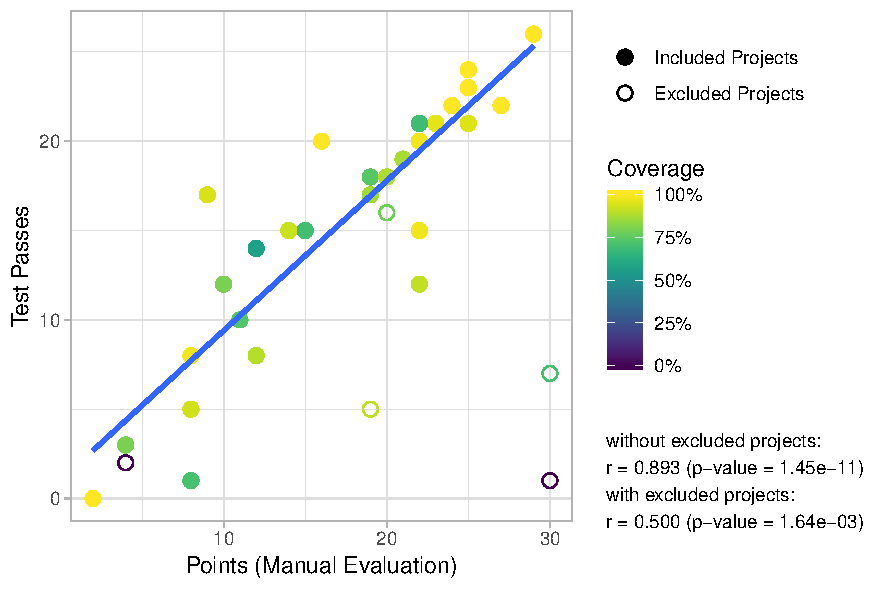
\includegraphics[width=\textwidth]{r/scatter-normal-1}
            \caption{Comparison between results of normal tests and manual scores, 1st run}
        \end{minipage}
    \end{figure}
\end{frame}

\begin{frame}\frametitle{Evaluation, Test Results, Normal Tests}
    \begin{figure}
        \begin{minipage}{.85\textwidth}
            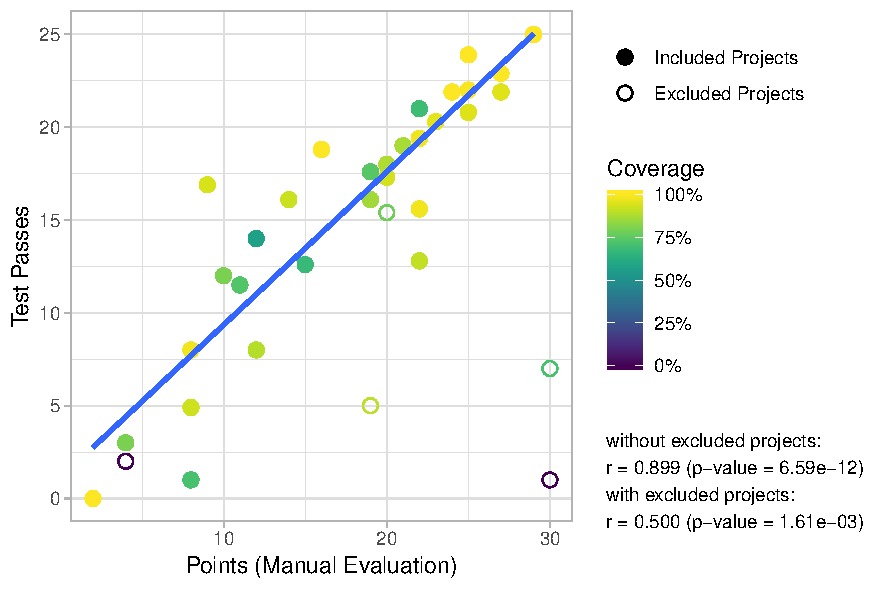
\includegraphics[width=\textwidth]{r/scatter-normal-avg}
            \caption{Comparison between results of normal tests and manual scores, average over 10 runs}
        \end{minipage}
    \end{figure}
\end{frame}

\begin{frame}\frametitle{Evaluation, Test Results, Constraint Tests}
    \begin{figure}
        \begin{minipage}{.85\textwidth}
            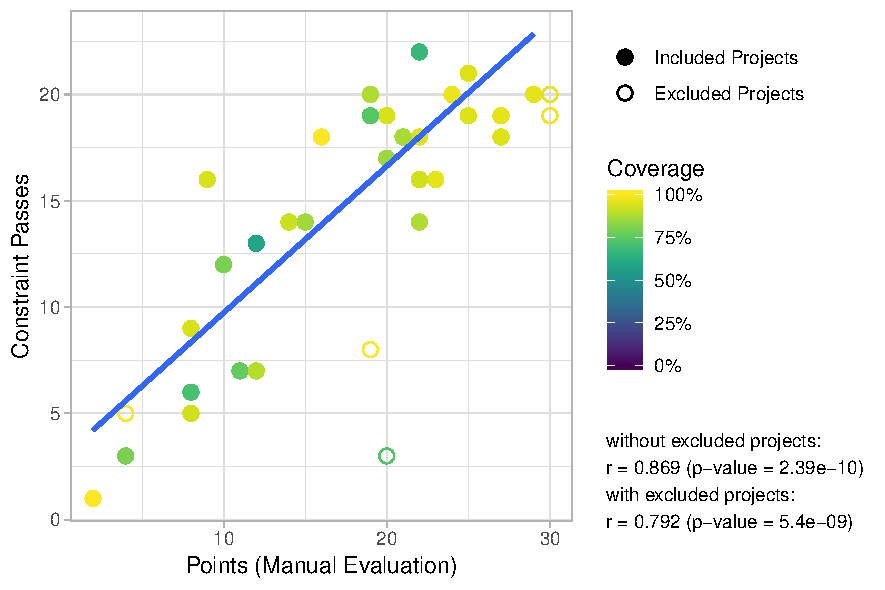
\includegraphics[width=\textwidth]{r/scatter-random-1}
            \caption{Comparison between results of constraint tests and manual scores, 1st run}
        \end{minipage}
    \end{figure}
\end{frame}

\begin{frame}\frametitle{Evaluation, Test Results, Constraint Tests}
    \begin{figure}
        \begin{minipage}{.85\textwidth}
            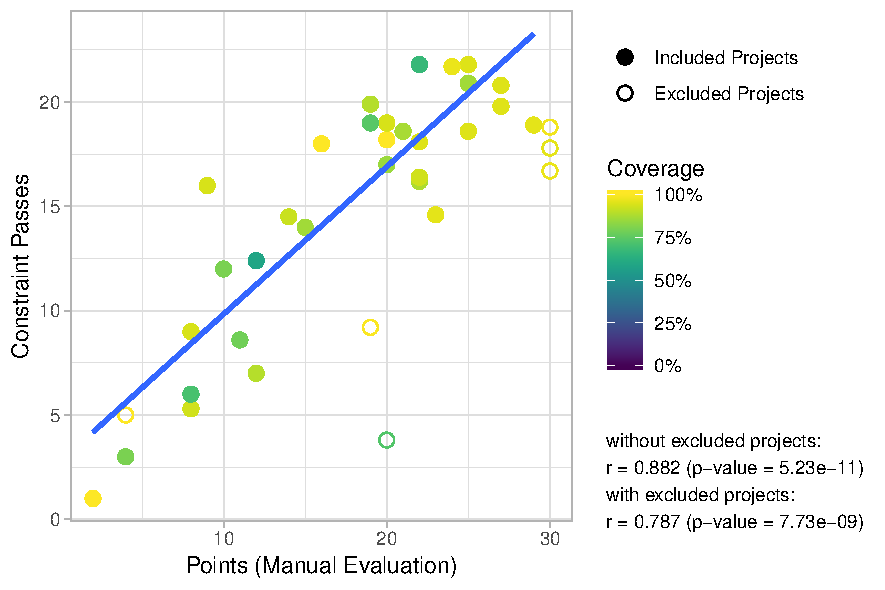
\includegraphics[width=\textwidth]{r/scatter-random-avg}
            \caption{Comparison between results of constraint tests and manual scores, average over 10 runs}
        \end{minipage}
    \end{figure}
\end{frame}

\begin{frame}
    \bigcenter{RQ: What coverage can be achieved with automated input?}
\end{frame}

\begin{frame}\frametitle{Evaluation, Coverage of Automated Input}
    Test subjects:
    \begin{itemize}
        \item 24 sample solutions to Code Club's\footnote{\url{https://codeclubprojects.org/}} online Scratch courses
        \item Run with generated input for 10 minutes
    \end{itemize}

    \pause
    \bigskip

    Measured item:
    \begin{itemize}
        \item Mean coverage of the projects after 10 minutes
        \item Coverage measured every second
    \end{itemize}
\end{frame}

\begin{frame}\frametitle{Evaluation, Coverage of Automated Input}
    \begin{figure}
        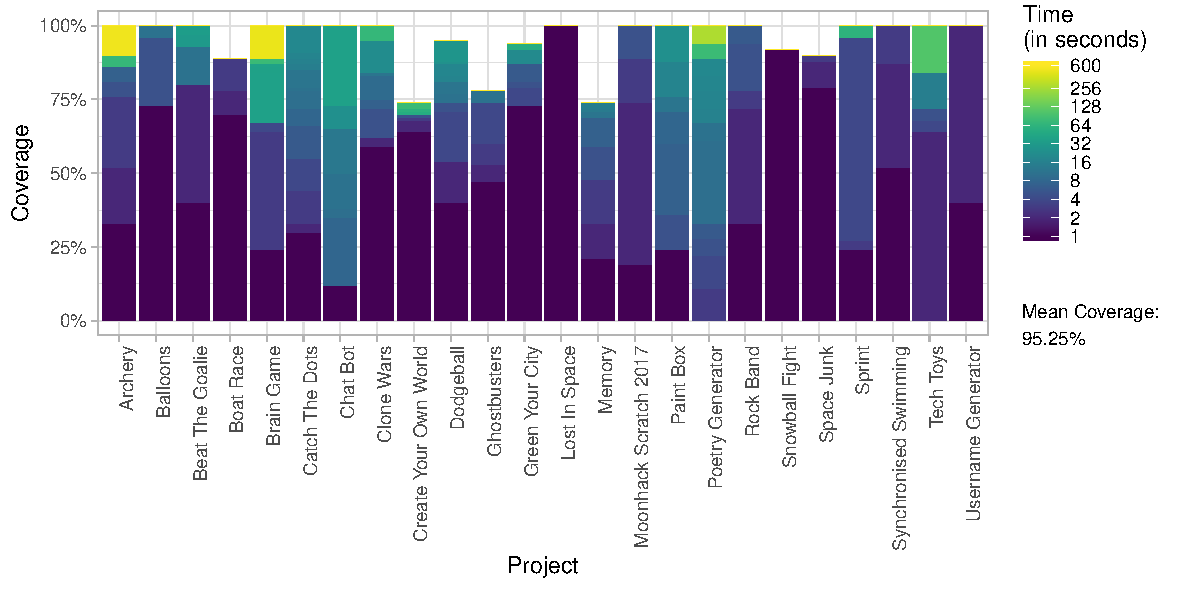
\includegraphics[width=\textwidth]{r/coverage-bar-random-input-1}
        \caption{Coverage per project, 1st run}
    \end{figure}
\end{frame}

\begin{frame}\frametitle{Evaluation, Coverage of Automated Input}
    \begin{figure}
        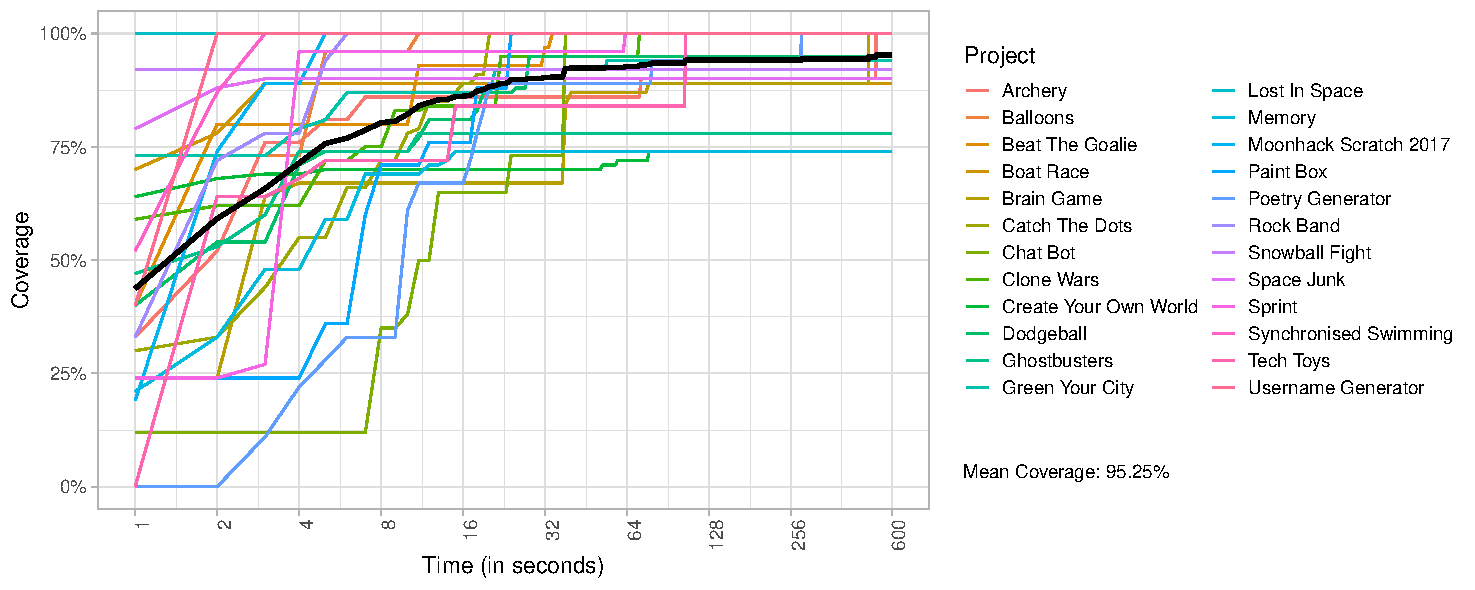
\includegraphics[width=\textwidth]{r/coverage-line-random-input-1}
        \caption{Coverage over time, 1st run}
    \end{figure}
\end{frame}

\begin{frame}\frametitle{Evaluation, Coverage of Automated Input}
    \begin{figure}
        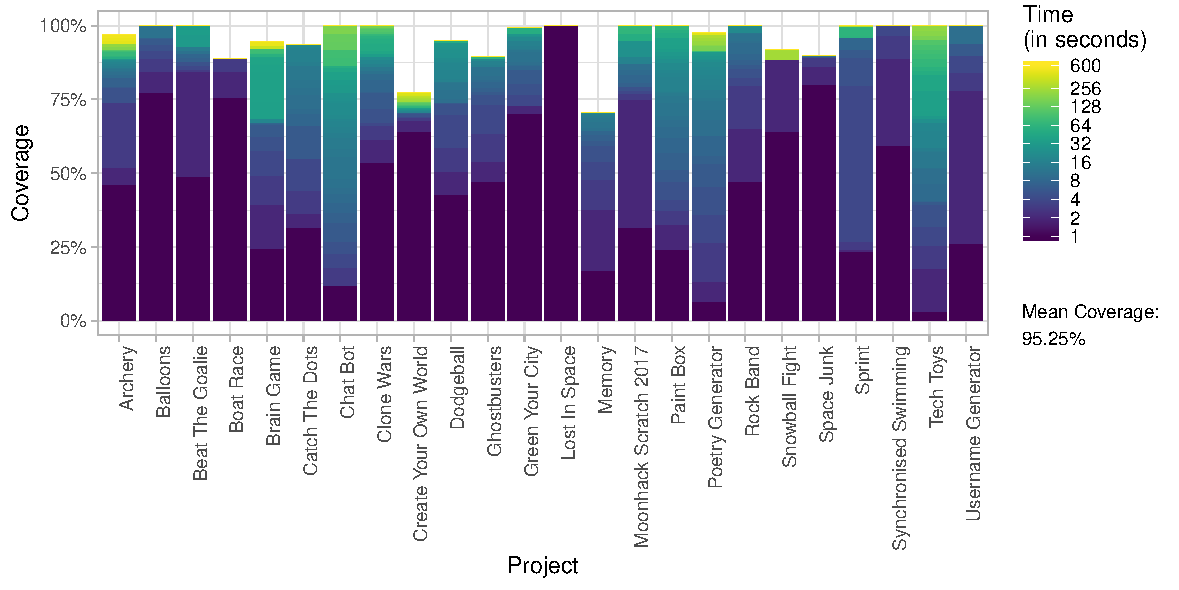
\includegraphics[width=\textwidth]{r/coverage-bar-random-input-avg}
        \caption{Coverage per project, average over 10 runs}
    \end{figure}
\end{frame}

\begin{frame}\frametitle{Evaluation, Coverage of Automated Input}
    \begin{figure}
        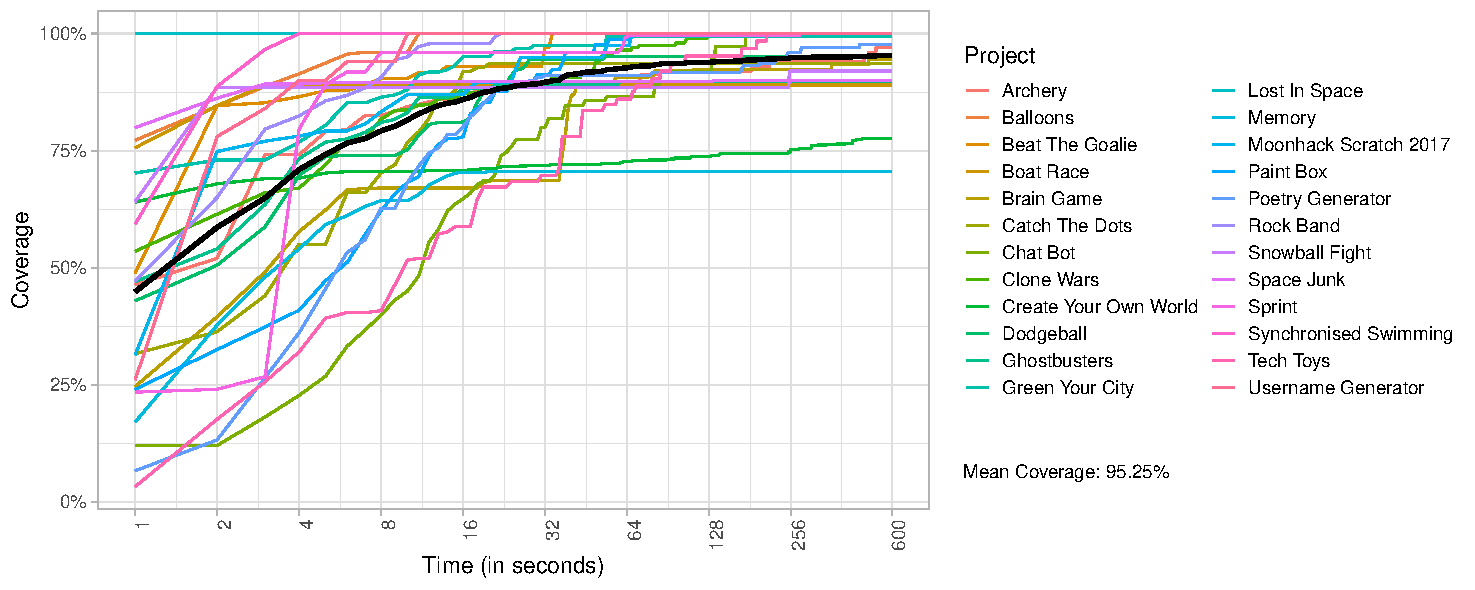
\includegraphics[width=\textwidth]{r/coverage-line-random-input-avg}
        \caption{Coverage over time, average over 10 runs}
    \end{figure}
\end{frame}

\begin{frame}\frametitle{Evaluation, Coverage of Automated Input}
    \begin{figure}
        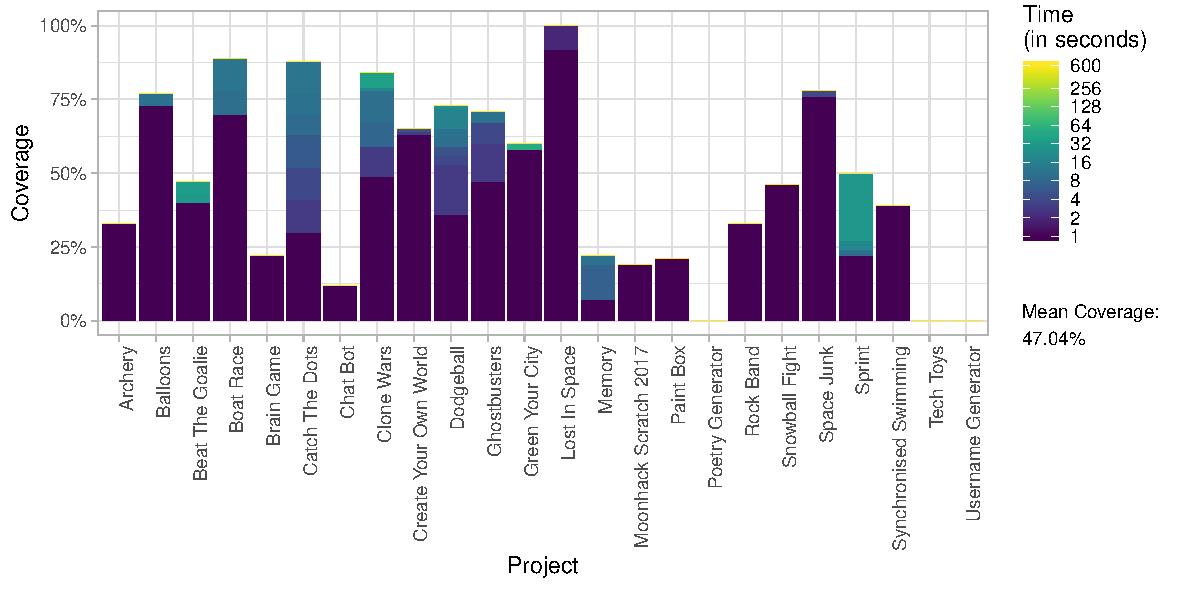
\includegraphics[width=\textwidth]{r/coverage-bar-no-input-1}
        \caption{Coverage per project, 1st run}
    \end{figure}
\end{frame}

\begin{frame}\frametitle{Evaluation, Coverage of Automated Input}
    \begin{figure}
        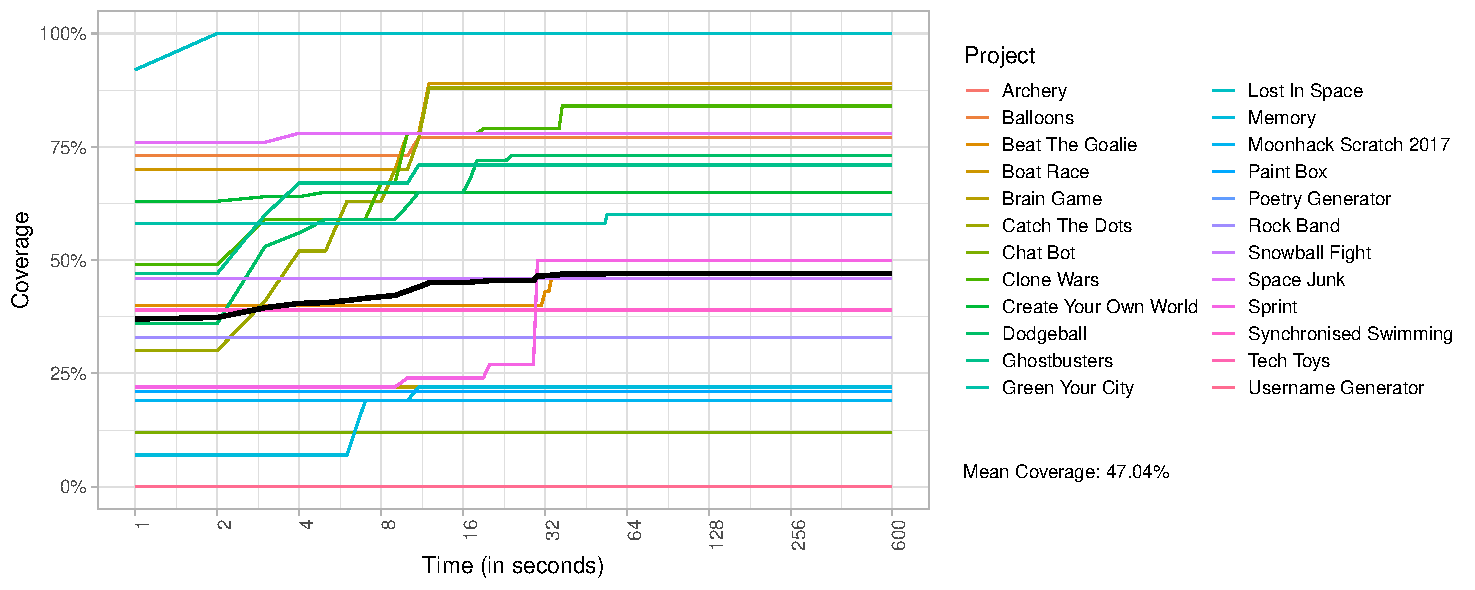
\includegraphics[width=\textwidth]{r/coverage-line-no-input-1}
        \caption{Coverage over time, 1st run}
    \end{figure}
\end{frame}

\begin{frame}\frametitle{Evaluation, Coverage of Automated Input}
    \begin{figure}
        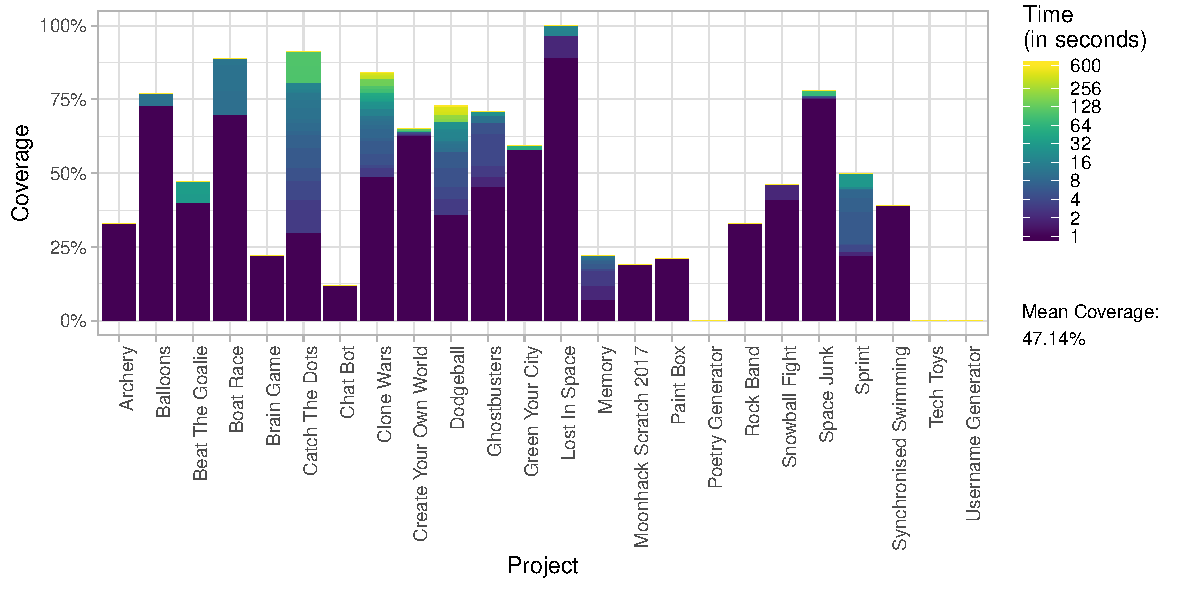
\includegraphics[width=\textwidth]{r/coverage-bar-no-input-avg}
        \caption{Coverage per project, average over 10 runs}
    \end{figure}
\end{frame}

\begin{frame}\frametitle{Evaluation, Coverage of Automated Input}
    \begin{figure}
        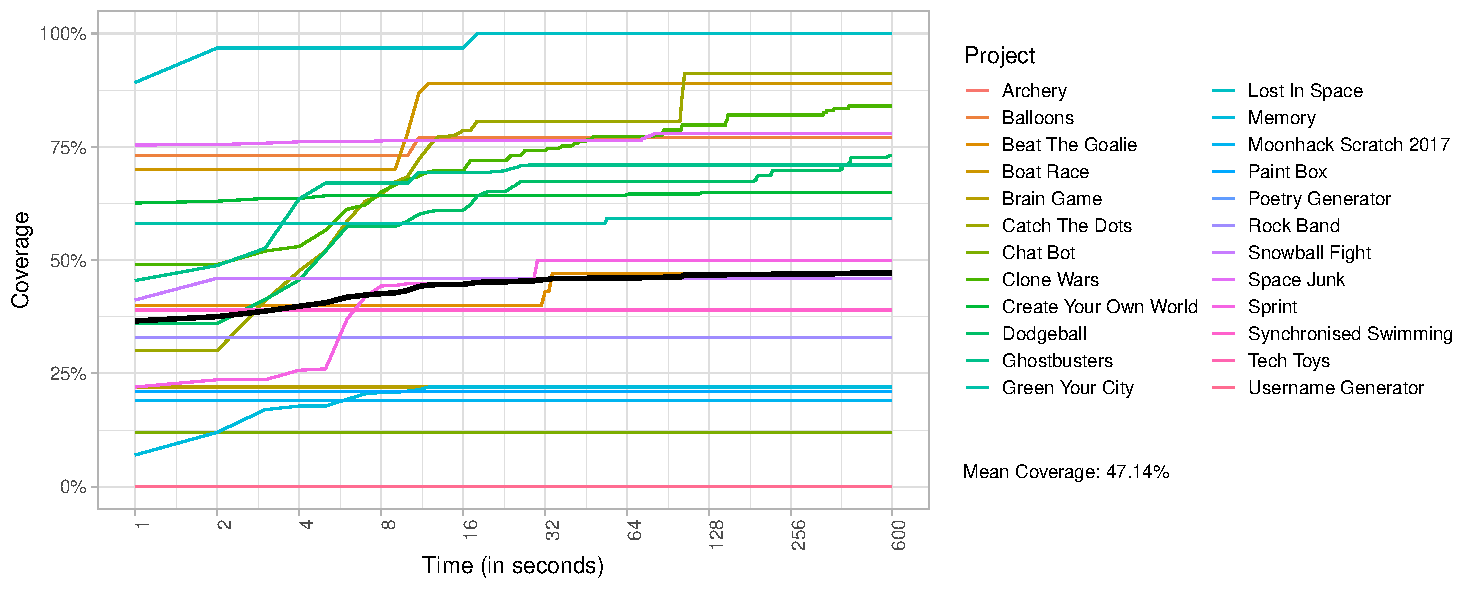
\includegraphics[width=\textwidth]{r/coverage-line-no-input-avg}
        \caption{Coverage over time, average over 10 runs}
    \end{figure}
\end{frame}


\end{document}
